
% Default to the notebook output style

    


% Inherit from the specified cell style.




    
\documentclass[11pt]{article}

    
    
    \usepackage[T1]{fontenc}
    % Nicer default font (+ math font) than Computer Modern for most use cases
    \usepackage{mathpazo}

    % Basic figure setup, for now with no caption control since it's done
    % automatically by Pandoc (which extracts ![](path) syntax from Markdown).
    \usepackage{graphicx}
    % We will generate all images so they have a width \maxwidth. This means
    % that they will get their normal width if they fit onto the page, but
    % are scaled down if they would overflow the margins.
    \makeatletter
    \def\maxwidth{\ifdim\Gin@nat@width>\linewidth\linewidth
    \else\Gin@nat@width\fi}
    \makeatother
    \let\Oldincludegraphics\includegraphics
    % Set max figure width to be 80% of text width, for now hardcoded.
    \renewcommand{\includegraphics}[1]{\Oldincludegraphics[width=.8\maxwidth]{#1}}
    % Ensure that by default, figures have no caption (until we provide a
    % proper Figure object with a Caption API and a way to capture that
    % in the conversion process - todo).
    \usepackage{caption}
    \DeclareCaptionLabelFormat{nolabel}{}
    \captionsetup{labelformat=nolabel}

    \usepackage{adjustbox} % Used to constrain images to a maximum size 
    \usepackage{xcolor} % Allow colors to be defined
    \usepackage{enumerate} % Needed for markdown enumerations to work
    \usepackage{geometry} % Used to adjust the document margins
    \usepackage{amsmath} % Equations
    \usepackage{amssymb} % Equations
    \usepackage{textcomp} % defines textquotesingle
    % Hack from http://tex.stackexchange.com/a/47451/13684:
    \AtBeginDocument{%
        \def\PYZsq{\textquotesingle}% Upright quotes in Pygmentized code
    }
    \usepackage{upquote} % Upright quotes for verbatim code
    \usepackage{eurosym} % defines \euro
    \usepackage[mathletters]{ucs} % Extended unicode (utf-8) support
    \usepackage[utf8x]{inputenc} % Allow utf-8 characters in the tex document
    \usepackage{fancyvrb} % verbatim replacement that allows latex
    \usepackage{grffile} % extends the file name processing of package graphics 
                         % to support a larger range 
    % The hyperref package gives us a pdf with properly built
    % internal navigation ('pdf bookmarks' for the table of contents,
    % internal cross-reference links, web links for URLs, etc.)
    \usepackage{hyperref}
    \usepackage{longtable} % longtable support required by pandoc >1.10
    \usepackage{booktabs}  % table support for pandoc > 1.12.2
    \usepackage[inline]{enumitem} % IRkernel/repr support (it uses the enumerate* environment)
    \usepackage[normalem]{ulem} % ulem is needed to support strikethroughs (\sout)
                                % normalem makes italics be italics, not underlines
    

    
    
    % Colors for the hyperref package
    \definecolor{urlcolor}{rgb}{0,.145,.698}
    \definecolor{linkcolor}{rgb}{.71,0.21,0.01}
    \definecolor{citecolor}{rgb}{.12,.54,.11}

    % ANSI colors
    \definecolor{ansi-black}{HTML}{3E424D}
    \definecolor{ansi-black-intense}{HTML}{282C36}
    \definecolor{ansi-red}{HTML}{E75C58}
    \definecolor{ansi-red-intense}{HTML}{B22B31}
    \definecolor{ansi-green}{HTML}{00A250}
    \definecolor{ansi-green-intense}{HTML}{007427}
    \definecolor{ansi-yellow}{HTML}{DDB62B}
    \definecolor{ansi-yellow-intense}{HTML}{B27D12}
    \definecolor{ansi-blue}{HTML}{208FFB}
    \definecolor{ansi-blue-intense}{HTML}{0065CA}
    \definecolor{ansi-magenta}{HTML}{D160C4}
    \definecolor{ansi-magenta-intense}{HTML}{A03196}
    \definecolor{ansi-cyan}{HTML}{60C6C8}
    \definecolor{ansi-cyan-intense}{HTML}{258F8F}
    \definecolor{ansi-white}{HTML}{C5C1B4}
    \definecolor{ansi-white-intense}{HTML}{A1A6B2}

    % commands and environments needed by pandoc snippets
    % extracted from the output of `pandoc -s`
    \providecommand{\tightlist}{%
      \setlength{\itemsep}{0pt}\setlength{\parskip}{0pt}}
    \DefineVerbatimEnvironment{Highlighting}{Verbatim}{commandchars=\\\{\}}
    % Add ',fontsize=\small' for more characters per line
    \newenvironment{Shaded}{}{}
    \newcommand{\KeywordTok}[1]{\textcolor[rgb]{0.00,0.44,0.13}{\textbf{{#1}}}}
    \newcommand{\DataTypeTok}[1]{\textcolor[rgb]{0.56,0.13,0.00}{{#1}}}
    \newcommand{\DecValTok}[1]{\textcolor[rgb]{0.25,0.63,0.44}{{#1}}}
    \newcommand{\BaseNTok}[1]{\textcolor[rgb]{0.25,0.63,0.44}{{#1}}}
    \newcommand{\FloatTok}[1]{\textcolor[rgb]{0.25,0.63,0.44}{{#1}}}
    \newcommand{\CharTok}[1]{\textcolor[rgb]{0.25,0.44,0.63}{{#1}}}
    \newcommand{\StringTok}[1]{\textcolor[rgb]{0.25,0.44,0.63}{{#1}}}
    \newcommand{\CommentTok}[1]{\textcolor[rgb]{0.38,0.63,0.69}{\textit{{#1}}}}
    \newcommand{\OtherTok}[1]{\textcolor[rgb]{0.00,0.44,0.13}{{#1}}}
    \newcommand{\AlertTok}[1]{\textcolor[rgb]{1.00,0.00,0.00}{\textbf{{#1}}}}
    \newcommand{\FunctionTok}[1]{\textcolor[rgb]{0.02,0.16,0.49}{{#1}}}
    \newcommand{\RegionMarkerTok}[1]{{#1}}
    \newcommand{\ErrorTok}[1]{\textcolor[rgb]{1.00,0.00,0.00}{\textbf{{#1}}}}
    \newcommand{\NormalTok}[1]{{#1}}
    
    % Additional commands for more recent versions of Pandoc
    \newcommand{\ConstantTok}[1]{\textcolor[rgb]{0.53,0.00,0.00}{{#1}}}
    \newcommand{\SpecialCharTok}[1]{\textcolor[rgb]{0.25,0.44,0.63}{{#1}}}
    \newcommand{\VerbatimStringTok}[1]{\textcolor[rgb]{0.25,0.44,0.63}{{#1}}}
    \newcommand{\SpecialStringTok}[1]{\textcolor[rgb]{0.73,0.40,0.53}{{#1}}}
    \newcommand{\ImportTok}[1]{{#1}}
    \newcommand{\DocumentationTok}[1]{\textcolor[rgb]{0.73,0.13,0.13}{\textit{{#1}}}}
    \newcommand{\AnnotationTok}[1]{\textcolor[rgb]{0.38,0.63,0.69}{\textbf{\textit{{#1}}}}}
    \newcommand{\CommentVarTok}[1]{\textcolor[rgb]{0.38,0.63,0.69}{\textbf{\textit{{#1}}}}}
    \newcommand{\VariableTok}[1]{\textcolor[rgb]{0.10,0.09,0.49}{{#1}}}
    \newcommand{\ControlFlowTok}[1]{\textcolor[rgb]{0.00,0.44,0.13}{\textbf{{#1}}}}
    \newcommand{\OperatorTok}[1]{\textcolor[rgb]{0.40,0.40,0.40}{{#1}}}
    \newcommand{\BuiltInTok}[1]{{#1}}
    \newcommand{\ExtensionTok}[1]{{#1}}
    \newcommand{\PreprocessorTok}[1]{\textcolor[rgb]{0.74,0.48,0.00}{{#1}}}
    \newcommand{\AttributeTok}[1]{\textcolor[rgb]{0.49,0.56,0.16}{{#1}}}
    \newcommand{\InformationTok}[1]{\textcolor[rgb]{0.38,0.63,0.69}{\textbf{\textit{{#1}}}}}
    \newcommand{\WarningTok}[1]{\textcolor[rgb]{0.38,0.63,0.69}{\textbf{\textit{{#1}}}}}
    
    
    % Define a nice break command that doesn't care if a line doesn't already
    % exist.
    \def\br{\hspace*{\fill} \\* }
    % Math Jax compatability definitions
    \def\gt{>}
    \def\lt{<}
    % Document parameters
    \title{tutorial}
    
    
    

    % Pygments definitions
    
\makeatletter
\def\PY@reset{\let\PY@it=\relax \let\PY@bf=\relax%
    \let\PY@ul=\relax \let\PY@tc=\relax%
    \let\PY@bc=\relax \let\PY@ff=\relax}
\def\PY@tok#1{\csname PY@tok@#1\endcsname}
\def\PY@toks#1+{\ifx\relax#1\empty\else%
    \PY@tok{#1}\expandafter\PY@toks\fi}
\def\PY@do#1{\PY@bc{\PY@tc{\PY@ul{%
    \PY@it{\PY@bf{\PY@ff{#1}}}}}}}
\def\PY#1#2{\PY@reset\PY@toks#1+\relax+\PY@do{#2}}

\expandafter\def\csname PY@tok@gd\endcsname{\def\PY@tc##1{\textcolor[rgb]{0.63,0.00,0.00}{##1}}}
\expandafter\def\csname PY@tok@gu\endcsname{\let\PY@bf=\textbf\def\PY@tc##1{\textcolor[rgb]{0.50,0.00,0.50}{##1}}}
\expandafter\def\csname PY@tok@gt\endcsname{\def\PY@tc##1{\textcolor[rgb]{0.00,0.27,0.87}{##1}}}
\expandafter\def\csname PY@tok@gs\endcsname{\let\PY@bf=\textbf}
\expandafter\def\csname PY@tok@gr\endcsname{\def\PY@tc##1{\textcolor[rgb]{1.00,0.00,0.00}{##1}}}
\expandafter\def\csname PY@tok@cm\endcsname{\let\PY@it=\textit\def\PY@tc##1{\textcolor[rgb]{0.25,0.50,0.50}{##1}}}
\expandafter\def\csname PY@tok@vg\endcsname{\def\PY@tc##1{\textcolor[rgb]{0.10,0.09,0.49}{##1}}}
\expandafter\def\csname PY@tok@vi\endcsname{\def\PY@tc##1{\textcolor[rgb]{0.10,0.09,0.49}{##1}}}
\expandafter\def\csname PY@tok@vm\endcsname{\def\PY@tc##1{\textcolor[rgb]{0.10,0.09,0.49}{##1}}}
\expandafter\def\csname PY@tok@mh\endcsname{\def\PY@tc##1{\textcolor[rgb]{0.40,0.40,0.40}{##1}}}
\expandafter\def\csname PY@tok@cs\endcsname{\let\PY@it=\textit\def\PY@tc##1{\textcolor[rgb]{0.25,0.50,0.50}{##1}}}
\expandafter\def\csname PY@tok@ge\endcsname{\let\PY@it=\textit}
\expandafter\def\csname PY@tok@vc\endcsname{\def\PY@tc##1{\textcolor[rgb]{0.10,0.09,0.49}{##1}}}
\expandafter\def\csname PY@tok@il\endcsname{\def\PY@tc##1{\textcolor[rgb]{0.40,0.40,0.40}{##1}}}
\expandafter\def\csname PY@tok@go\endcsname{\def\PY@tc##1{\textcolor[rgb]{0.53,0.53,0.53}{##1}}}
\expandafter\def\csname PY@tok@cp\endcsname{\def\PY@tc##1{\textcolor[rgb]{0.74,0.48,0.00}{##1}}}
\expandafter\def\csname PY@tok@gi\endcsname{\def\PY@tc##1{\textcolor[rgb]{0.00,0.63,0.00}{##1}}}
\expandafter\def\csname PY@tok@gh\endcsname{\let\PY@bf=\textbf\def\PY@tc##1{\textcolor[rgb]{0.00,0.00,0.50}{##1}}}
\expandafter\def\csname PY@tok@ni\endcsname{\let\PY@bf=\textbf\def\PY@tc##1{\textcolor[rgb]{0.60,0.60,0.60}{##1}}}
\expandafter\def\csname PY@tok@nl\endcsname{\def\PY@tc##1{\textcolor[rgb]{0.63,0.63,0.00}{##1}}}
\expandafter\def\csname PY@tok@nn\endcsname{\let\PY@bf=\textbf\def\PY@tc##1{\textcolor[rgb]{0.00,0.00,1.00}{##1}}}
\expandafter\def\csname PY@tok@no\endcsname{\def\PY@tc##1{\textcolor[rgb]{0.53,0.00,0.00}{##1}}}
\expandafter\def\csname PY@tok@na\endcsname{\def\PY@tc##1{\textcolor[rgb]{0.49,0.56,0.16}{##1}}}
\expandafter\def\csname PY@tok@nb\endcsname{\def\PY@tc##1{\textcolor[rgb]{0.00,0.50,0.00}{##1}}}
\expandafter\def\csname PY@tok@nc\endcsname{\let\PY@bf=\textbf\def\PY@tc##1{\textcolor[rgb]{0.00,0.00,1.00}{##1}}}
\expandafter\def\csname PY@tok@nd\endcsname{\def\PY@tc##1{\textcolor[rgb]{0.67,0.13,1.00}{##1}}}
\expandafter\def\csname PY@tok@ne\endcsname{\let\PY@bf=\textbf\def\PY@tc##1{\textcolor[rgb]{0.82,0.25,0.23}{##1}}}
\expandafter\def\csname PY@tok@nf\endcsname{\def\PY@tc##1{\textcolor[rgb]{0.00,0.00,1.00}{##1}}}
\expandafter\def\csname PY@tok@si\endcsname{\let\PY@bf=\textbf\def\PY@tc##1{\textcolor[rgb]{0.73,0.40,0.53}{##1}}}
\expandafter\def\csname PY@tok@s2\endcsname{\def\PY@tc##1{\textcolor[rgb]{0.73,0.13,0.13}{##1}}}
\expandafter\def\csname PY@tok@nt\endcsname{\let\PY@bf=\textbf\def\PY@tc##1{\textcolor[rgb]{0.00,0.50,0.00}{##1}}}
\expandafter\def\csname PY@tok@nv\endcsname{\def\PY@tc##1{\textcolor[rgb]{0.10,0.09,0.49}{##1}}}
\expandafter\def\csname PY@tok@s1\endcsname{\def\PY@tc##1{\textcolor[rgb]{0.73,0.13,0.13}{##1}}}
\expandafter\def\csname PY@tok@dl\endcsname{\def\PY@tc##1{\textcolor[rgb]{0.73,0.13,0.13}{##1}}}
\expandafter\def\csname PY@tok@ch\endcsname{\let\PY@it=\textit\def\PY@tc##1{\textcolor[rgb]{0.25,0.50,0.50}{##1}}}
\expandafter\def\csname PY@tok@m\endcsname{\def\PY@tc##1{\textcolor[rgb]{0.40,0.40,0.40}{##1}}}
\expandafter\def\csname PY@tok@gp\endcsname{\let\PY@bf=\textbf\def\PY@tc##1{\textcolor[rgb]{0.00,0.00,0.50}{##1}}}
\expandafter\def\csname PY@tok@sh\endcsname{\def\PY@tc##1{\textcolor[rgb]{0.73,0.13,0.13}{##1}}}
\expandafter\def\csname PY@tok@ow\endcsname{\let\PY@bf=\textbf\def\PY@tc##1{\textcolor[rgb]{0.67,0.13,1.00}{##1}}}
\expandafter\def\csname PY@tok@sx\endcsname{\def\PY@tc##1{\textcolor[rgb]{0.00,0.50,0.00}{##1}}}
\expandafter\def\csname PY@tok@bp\endcsname{\def\PY@tc##1{\textcolor[rgb]{0.00,0.50,0.00}{##1}}}
\expandafter\def\csname PY@tok@c1\endcsname{\let\PY@it=\textit\def\PY@tc##1{\textcolor[rgb]{0.25,0.50,0.50}{##1}}}
\expandafter\def\csname PY@tok@fm\endcsname{\def\PY@tc##1{\textcolor[rgb]{0.00,0.00,1.00}{##1}}}
\expandafter\def\csname PY@tok@o\endcsname{\def\PY@tc##1{\textcolor[rgb]{0.40,0.40,0.40}{##1}}}
\expandafter\def\csname PY@tok@kc\endcsname{\let\PY@bf=\textbf\def\PY@tc##1{\textcolor[rgb]{0.00,0.50,0.00}{##1}}}
\expandafter\def\csname PY@tok@c\endcsname{\let\PY@it=\textit\def\PY@tc##1{\textcolor[rgb]{0.25,0.50,0.50}{##1}}}
\expandafter\def\csname PY@tok@mf\endcsname{\def\PY@tc##1{\textcolor[rgb]{0.40,0.40,0.40}{##1}}}
\expandafter\def\csname PY@tok@err\endcsname{\def\PY@bc##1{\setlength{\fboxsep}{0pt}\fcolorbox[rgb]{1.00,0.00,0.00}{1,1,1}{\strut ##1}}}
\expandafter\def\csname PY@tok@mb\endcsname{\def\PY@tc##1{\textcolor[rgb]{0.40,0.40,0.40}{##1}}}
\expandafter\def\csname PY@tok@ss\endcsname{\def\PY@tc##1{\textcolor[rgb]{0.10,0.09,0.49}{##1}}}
\expandafter\def\csname PY@tok@sr\endcsname{\def\PY@tc##1{\textcolor[rgb]{0.73,0.40,0.53}{##1}}}
\expandafter\def\csname PY@tok@mo\endcsname{\def\PY@tc##1{\textcolor[rgb]{0.40,0.40,0.40}{##1}}}
\expandafter\def\csname PY@tok@kd\endcsname{\let\PY@bf=\textbf\def\PY@tc##1{\textcolor[rgb]{0.00,0.50,0.00}{##1}}}
\expandafter\def\csname PY@tok@mi\endcsname{\def\PY@tc##1{\textcolor[rgb]{0.40,0.40,0.40}{##1}}}
\expandafter\def\csname PY@tok@kn\endcsname{\let\PY@bf=\textbf\def\PY@tc##1{\textcolor[rgb]{0.00,0.50,0.00}{##1}}}
\expandafter\def\csname PY@tok@cpf\endcsname{\let\PY@it=\textit\def\PY@tc##1{\textcolor[rgb]{0.25,0.50,0.50}{##1}}}
\expandafter\def\csname PY@tok@kr\endcsname{\let\PY@bf=\textbf\def\PY@tc##1{\textcolor[rgb]{0.00,0.50,0.00}{##1}}}
\expandafter\def\csname PY@tok@s\endcsname{\def\PY@tc##1{\textcolor[rgb]{0.73,0.13,0.13}{##1}}}
\expandafter\def\csname PY@tok@kp\endcsname{\def\PY@tc##1{\textcolor[rgb]{0.00,0.50,0.00}{##1}}}
\expandafter\def\csname PY@tok@w\endcsname{\def\PY@tc##1{\textcolor[rgb]{0.73,0.73,0.73}{##1}}}
\expandafter\def\csname PY@tok@kt\endcsname{\def\PY@tc##1{\textcolor[rgb]{0.69,0.00,0.25}{##1}}}
\expandafter\def\csname PY@tok@sc\endcsname{\def\PY@tc##1{\textcolor[rgb]{0.73,0.13,0.13}{##1}}}
\expandafter\def\csname PY@tok@sb\endcsname{\def\PY@tc##1{\textcolor[rgb]{0.73,0.13,0.13}{##1}}}
\expandafter\def\csname PY@tok@sa\endcsname{\def\PY@tc##1{\textcolor[rgb]{0.73,0.13,0.13}{##1}}}
\expandafter\def\csname PY@tok@k\endcsname{\let\PY@bf=\textbf\def\PY@tc##1{\textcolor[rgb]{0.00,0.50,0.00}{##1}}}
\expandafter\def\csname PY@tok@se\endcsname{\let\PY@bf=\textbf\def\PY@tc##1{\textcolor[rgb]{0.73,0.40,0.13}{##1}}}
\expandafter\def\csname PY@tok@sd\endcsname{\let\PY@it=\textit\def\PY@tc##1{\textcolor[rgb]{0.73,0.13,0.13}{##1}}}

\def\PYZbs{\char`\\}
\def\PYZus{\char`\_}
\def\PYZob{\char`\{}
\def\PYZcb{\char`\}}
\def\PYZca{\char`\^}
\def\PYZam{\char`\&}
\def\PYZlt{\char`\<}
\def\PYZgt{\char`\>}
\def\PYZsh{\char`\#}
\def\PYZpc{\char`\%}
\def\PYZdl{\char`\$}
\def\PYZhy{\char`\-}
\def\PYZsq{\char`\'}
\def\PYZdq{\char`\"}
\def\PYZti{\char`\~}
% for compatibility with earlier versions
\def\PYZat{@}
\def\PYZlb{[}
\def\PYZrb{]}
\makeatother


    % Exact colors from NB
    \definecolor{incolor}{rgb}{0.0, 0.0, 0.5}
    \definecolor{outcolor}{rgb}{0.545, 0.0, 0.0}



    
    % Prevent overflowing lines due to hard-to-break entities
    \sloppy 
    % Setup hyperref package
    \hypersetup{
      breaklinks=true,  % so long urls are correctly broken across lines
      colorlinks=true,
      urlcolor=urlcolor,
      linkcolor=linkcolor,
      citecolor=citecolor,
      }
    % Slightly bigger margins than the latex defaults
    
    \geometry{verbose,tmargin=1in,bmargin=1in,lmargin=1in,rmargin=1in}
    
    

    \begin{document}
    
    
    \maketitle
    
    

    
    \section{The Grabow Group Handbook}\label{the-grabow-group-handbook}

Authors: Hari Thirumalai, Juan Manuel Arce-Ramos and Karun Kumar Rao

    \subsection{Introduction}\label{introduction}

The aim of this document is to help users who are new to the concepts
and tools used in the group. By the end of this tutorial, the reader
will should have a basic understanding of the various components of
typical computational research workflows, starting from basic Linux
commands to running calculations using VASP and other softwares. This
document was not designed to be a thorough guide and the user is
encourage to complement the information provided here with extensive
Google searches.

We also recommend you to look at John Kitchin's DFT Book
\href{http://kitchingroup.cheme.cmu.edu/dft-book/dft.pdf}{pdf} or
\href{http://kitchingroup.cheme.cmu.edu/dft-book/dft.html}{html}
versions since it contains many working examples that touch upon
practical concepts of computational catalysis which can be easily (or
relatively easy) followed and implemented.

    \subsection{High Performance
Computing}\label{high-performance-computing}

A significant portion of the research conducted in the group pertains to
computational modeling in which various properties of interest for a
system are calculated by means of /ab initio/ density functional theory
calculations. We refer the reader to an excellent
\href{https://www.wiley.com/en-us/Density+Functional+Theory\%3A+A+Practical+Introduction-p-9780470373170}{book}
that delves on the nuts and bolts of DFT by David Sholl. These
calculations are computationally intensive and are exclusively performed
on computing clusters or supercomputers. These massively-parallel
machines are accessed remotely through the
\href{https://www.ssh.com/ssh/protocol}{Secure Shell Protocol} and the
user is able to access his or her account on that machine. Once logged
in, the user sets up these jobs and submits them to the system's
resource manager, or the queue. Once resources become available, the
queue executes the job and the user is notified upon completion of the
job.

    \subsubsection{Queues}\label{queues}

The queue is a utility that accepts job submissions from users,
implements a fair use policy, and allocates resources based on job
requirements and other parameters. Most of the systems used by our group
are managed by the \href{http://slurm.schedmd.com/}{SLURM} Workload
Manager=. Maxwell is managed by the
\href{http://www.adaptivecomputing.com/products/open-source/torque/}{Torque
Resource Manager}. The configuration keywords and parameters are
different for different systems and every job submission script must
contain these parameters for it to be accepted by the queue. The queue
keywords are

    For =SLURM=

\begin{verbatim}
#SBATCH -p <queue partition>
#SBATCH -o myMPI.o%j
#SBATCH -N <number of nodes> -n <number of processors per node>
#SBATCH -t <walltime in hhh:mm:ss>
#SBATCH --mail-type=END
#SBATCH --mail-user=<user email id>
\end{verbatim}

For =Torque=

\begin{verbatim}
#PBS -e myMPI.e%j
#PBS -o myMPI.o%j
#PBS -m ae
#PBS -M <user email id> 
#PBS -l <walltime in hhh:mm:ss>
#PBS -r n
#PBS -l nodes=<number of nodes>:ppn=<number of processors per node>
#PBS -l pmem=<Memory requested per node in mb>
#PBS -S /bin/tcsh <Specify type of Shell>
\end{verbatim}

    A more detailed explanation of these parameters follows: - queue
partition: This specifies the partition to which you want to submit your
job. - number of nodes: A node is a group of processors, which are
designed to work together with maximum efficiency. A simple example of a
node would be a computer with an Intel i5 processor, where the single
node has 4 processors. - number of processors: This is the number of
processors or threads in a node. Usually, the user is expected to
request all processors in a node. This parameter is system configuration
dependent. - walltime in hours: This specifies the time until which the
job will execute on the system. Once runtime exceeds this value, the job
execution is terminated.

    \subsubsection{Jobscripts}\label{jobscripts}

Jobscripts are executable files of a defined environment which consist
of executable code. Jobscripts can be in a variety of file formats and
the most commonly used ones are python, shell and cshell jobscripts. A
jobscript and a simple file are differentiated by the file type
identifier. This line tells the compiler, interpreter and any
text-editor the type of the file. This removes the need for an extension
to the file, which can also serve as an identifier. A properly
identified file also enables source code formatting on text-editors.

Example job scripts for SLURM and PBS (toruque) schedulers are given
below

    \begin{verbatim}
#!/usr/bin/env python --> File environment identifier

#SBATCH -p batch
#SBATCH -o myMPI.o%j
#SBATCH -N 5 -n 100                            [SLURM Parameters]
#SBATCH -t 168:00:00
#SBATCH --mail-type=END
#SBATCH --mail-user=hthirumalai@gmail.com

# Your executable python code begins here
from ase.io import read
from ase.calculators.vasp import Vasp

...
\end{verbatim}

and

\begin{verbatim}
#!/usr/bin/env python

#PBS -e stderr
#PBS -o stdout
#PBS -m ae
#PBS -M hthirumalai@gmail.com
#PBS -l walltime=100:00:00
#PBS -r n                                        [PBS Parameters]
#PBS -l nodes=1:ppn=12
#PBS -l pmem=2500mb
#PBS -S /bin/tcsh
#PBS -V

from ase import *
from ase.calculators.vasp import Vasp

...
\end{verbatim}

    \begin{verbatim}
#!/bin/sh --> File environment identifier

#SBATCH -p batch
#SBATCH -o myMPI.o%j
#SBATCH -N 5 -n 100                            [SLURM Parameters]
#SBATCH -t 168:00:00
#SBATCH --mail-type=END
#SBATCH --mail-user=hthirumalai@gmail.com

# Your executable shell script begins here
echo 'VASP starting execution ..'

...
\end{verbatim}

and

\begin{verbatim}
#!/bin/sh

#PBS -e stderr
#PBS -o stdout
#PBS -m ae
#PBS -M mayerzmytm@gmail.com
#PBS -l walltime=100:00:00
#PBS -r n                                        [PBS Parameters]
#PBS -l nodes=1:ppn=12
#PBS -l pmem=2500mb
#PBS -S /bin/tcsh
#PBS -V

# Your executable shell script begins here
echo 'VASP starting execution ..'
\end{verbatim}

    \subsubsection{System Specific Settings}\label{system-specific-settings}

Our group has access to various clusters at any given time and job
scripts must be modified such that they execute without errors when
transferred from one cluster to another. This section consists of all
cluster relevant information. All storage-intensive jobs must be
executed on the group's project directories. These locations are
backed-up on a daily basis. \$SCRATCH directories on Cori and Stampede2
are short term, high I/O performance storage that are periodically
purged. Therefore, the reader is advised to use these directories for
running jobs only and transfer these files to permanent storage on the
University of Houston clusters.

    Opuntia

\begin{verbatim}
project directory: /project/grabow

#SBATCH -p grabow
#SBATCH -o myMPI.o%j   
#SBATCH -N 1 -n 20
#SBATCH -t 24:00:00
#SBATCH --mail-type=END
#SBATCH --mail-user=@gmail.com
\end{verbatim}

uHPC

\begin{verbatim}
project directory: /uhpc/grabow

#SBATCH -p batch
#SBATCH -o myMPI.o%j   
#SBATCH -N 1 -n 20
#SBATCH -t 24:00:00
#SBATCH --mail-type=END
#SBATCH --mail-user=@gmail.com  
\end{verbatim}

Juniper

\begin{verbatim}
project directory: /project/grabow

#SBATCH -p batch
#SBATCH -o myMPI.o%j   
#SBATCH -N 1 -n 24
#SBATCH -t 24:00:00
#SBATCH --mail-type=END
#SBATCH --mail-user=@gmail.com 
\end{verbatim}

Sabine

\begin{verbatim}
project directory: /brazos/grabow

#SBATCH -p batch
#SBATCH -o myMPI.o%j   
#SBATCH -N 1 -n 24
#SBATCH -t 24:00:00
#SBATCH --mail-type=END
#SBATCH --mail-user=@gmail.com  
\end{verbatim}

Cori

\begin{verbatim}
scratch directory: $SCRATCH
project directory: /global/project/projectdirs/m2029/

#SBATCH -p regular
#SBATCH -C knl
#SBATCH -A m2029
#SBATCH -o myMPI.o%j   
#SBATCH -N 1 -n 64
#SBATCH -t 24:00:00
#SBATCH --mail-type=END
#SBATCH --mail-user=@gmail.com  
\end{verbatim}

AND

\begin{verbatim}
#SBATCH -p regular
#SBATCH -C haswell
#SBATCH -A m2029
#SBATCH -o myMPI.o%j   
#SBATCH -N 1 -n 32
#SBATCH -t 24:00:00
#SBATCH --mail-type=END
#SBATCH --mail-user=@gmail.com  
\end{verbatim}

Stampede2

\begin{verbatim}
scratch directory: $SCRATCH
project directory: $WORK

#SBATCH -p normal
#SBATCH -o myMPI.o%j   
#SBATCH -N 1 -n 64
#SBATCH -t 24:00:00
#SBATCH --mail-type=END
#SBATCH --mail-user=@gmail.com  
\end{verbatim}

AND

\begin{verbatim}
#SBATCH -p skx-normal
#SBATCH -o myMPI.o%j   
#SBATCH -N 1 -n 48
#SBATCH -t 24:00:00
#SBATCH --mail-type=END
#SBATCH --mail-user=@gmail.com  
\end{verbatim}

    \subsubsection{Terminals}\label{terminals}

The terminal is the application that allows the user to interact with
the computer through the command line. Any output from code can also be
piped out to the command line on the terminal.

A Windows user needs to download software that provides a terminal for
remote ssh access and Linux and Mac OS users can use the pre-installed
terminal on their computer. The figure that follows shows a typical
terminal window on a Mac OS computer. Users can access the terminals by
searching for =Terminal= in Apple's Spotlight Search (command+space).

\begin{figure}
\centering
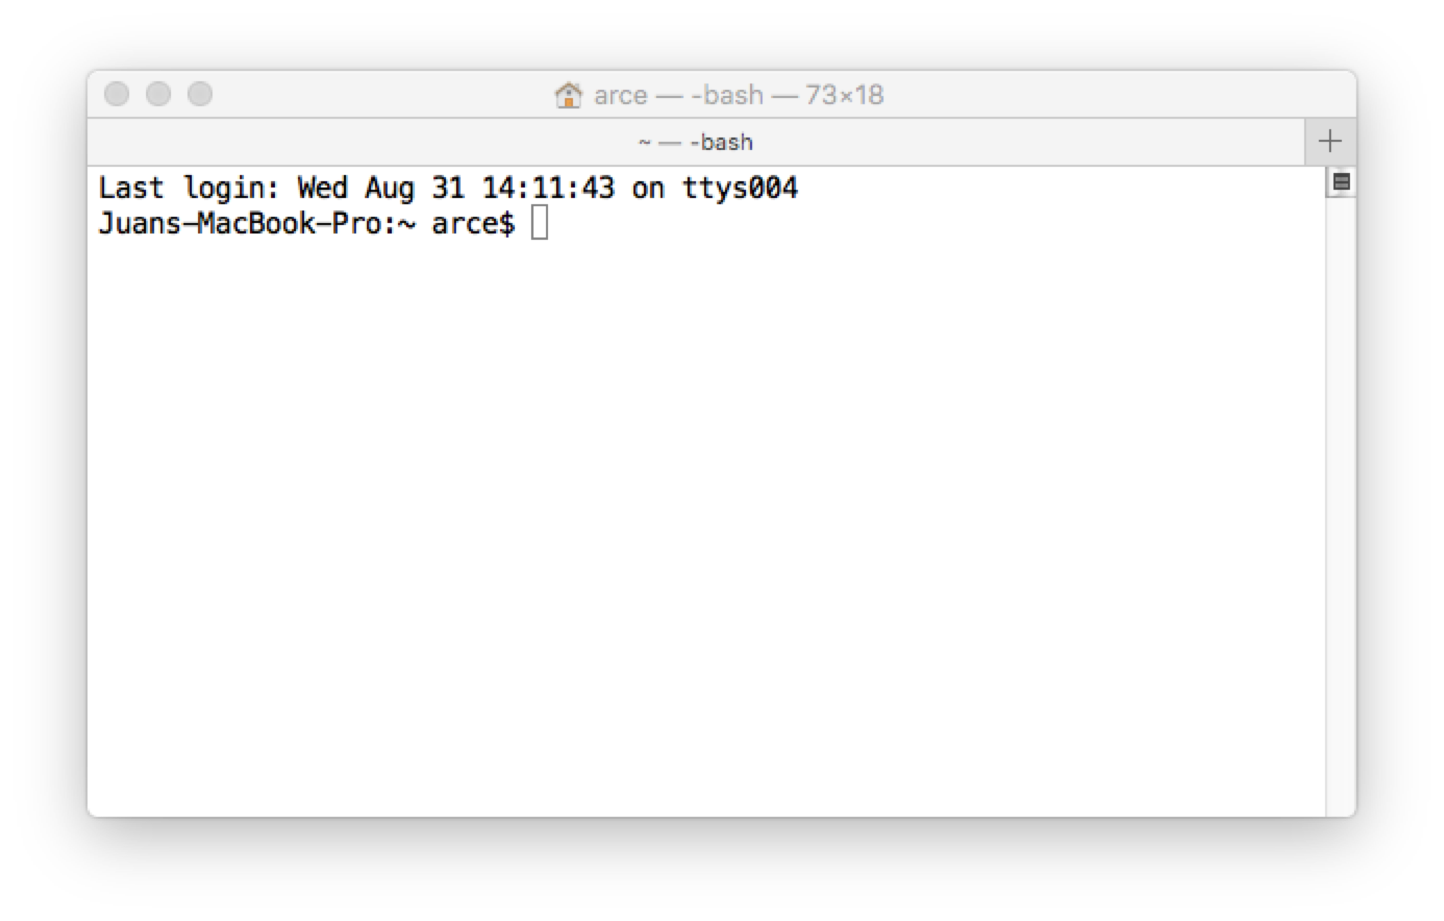
\includegraphics{figures/terminal-mac.png}
\caption{Terminal window on Mac OS}
\end{figure}

If you are a Linux user then you should be able to start a terminal
without the need for any installation. Terminal on a Linux system
running Ubuntu can be accessed using Ctrl+Alt+T. Multiple tabs can be
opened by hitting Ctrl+Shift+T.

\begin{figure}
\centering
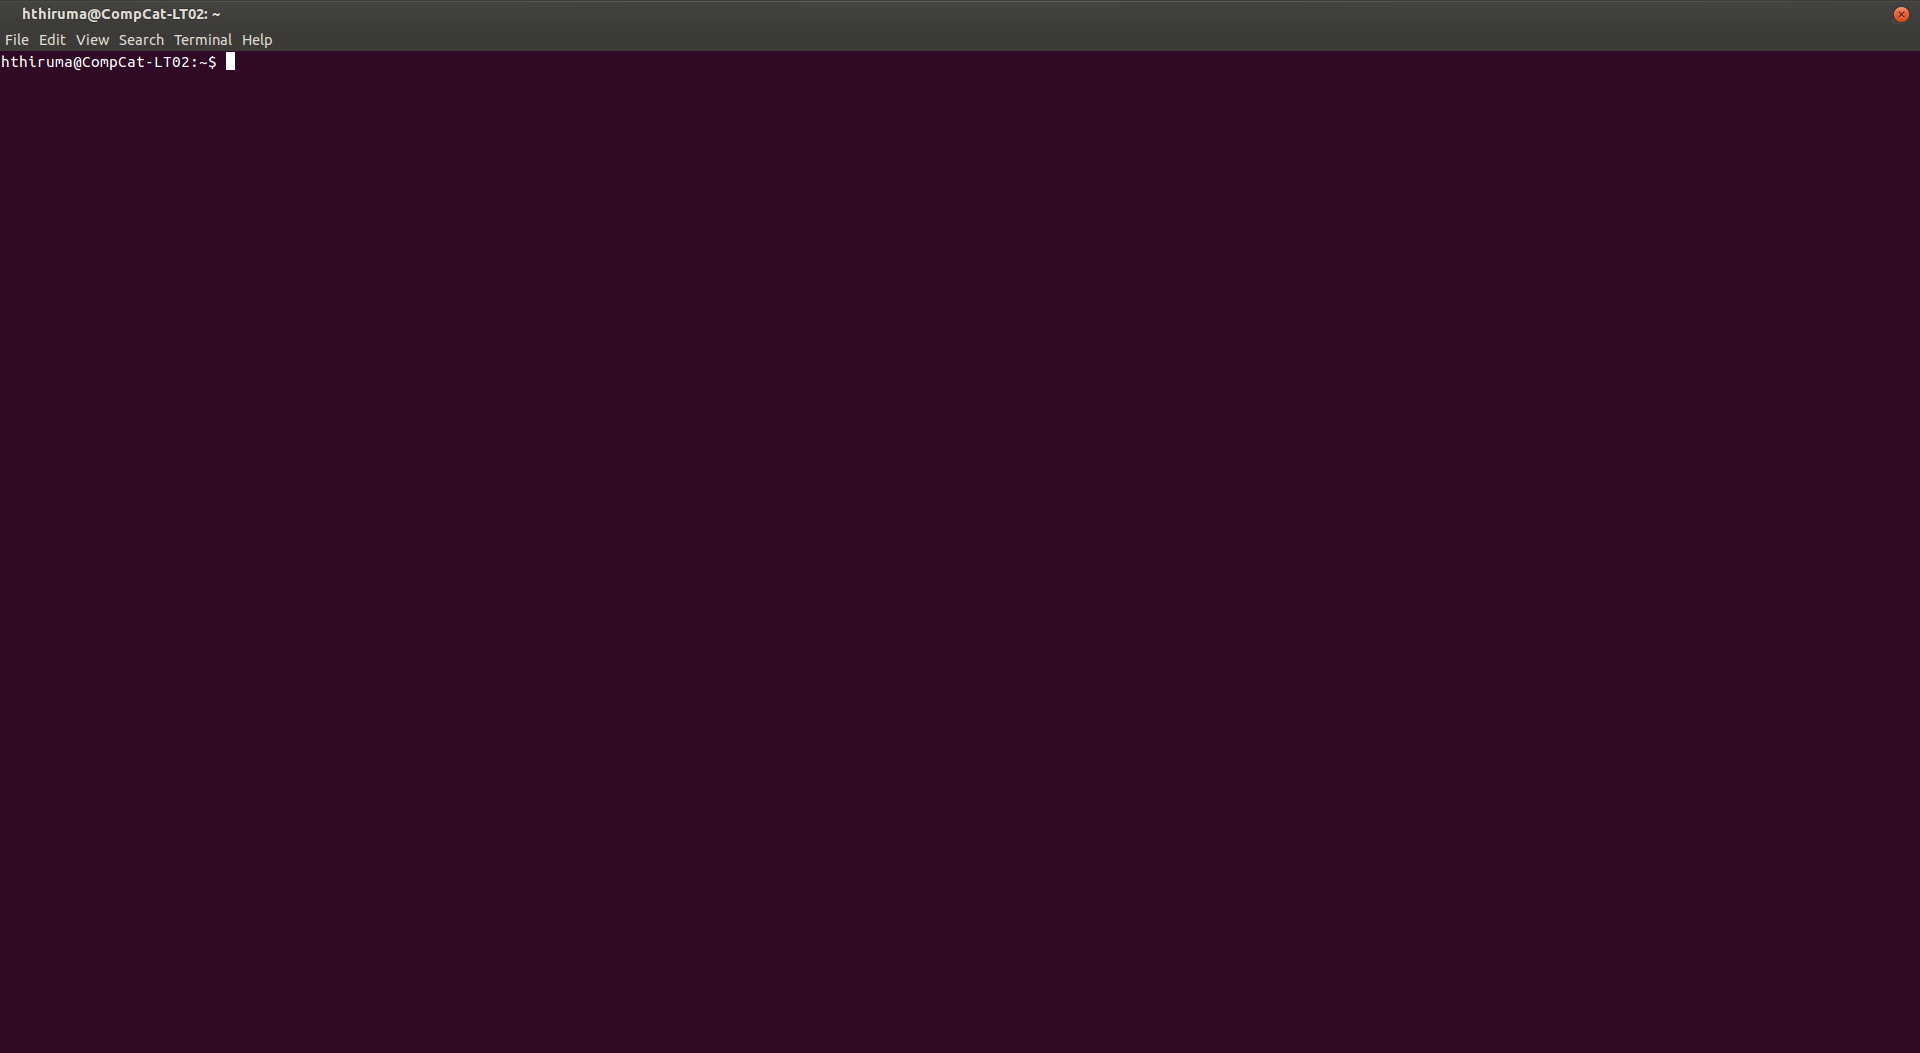
\includegraphics{figures/Ubuntu-terminal.png}
\caption{Terminal window on Linux}
\end{figure}

Windows users can install either
\href{http://mobaxterm.mobatek.net/}{MobaXTerm} or
\href{http://www.straightrunning.com/XmingNotes/}{Xming}. We recommend
MobaXTerm.

\begin{figure}
\centering
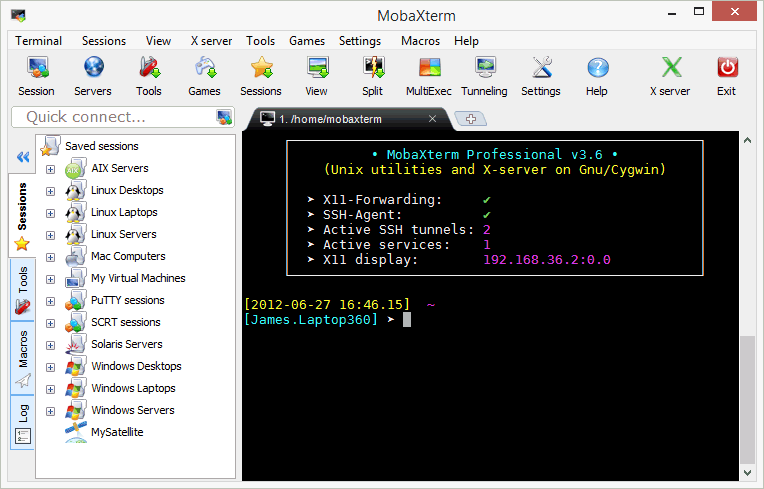
\includegraphics{figures/moba.png}
\caption{MobaXTerm Terminal window on Windows}
\end{figure}

    \subsubsection{Logging into
clusters/supercomputers}\label{logging-into-clusterssupercomputers}

In order to login into your account in a cluster or supercomputer you
need the address of the remote machine and have an account in it. One
should be able to connect to the remote computer typing the following
command in a terminal

\begin{verbatim}
ssh -X user_name@supercomputer_address
\end{verbatim}

Addresses of the supercomputers used by the group are

\begin{verbatim}
System: colossus
Address: colossus.egr.uh.edu

System: opuntia
Address: opuntia.cacds.uh.edu

System: maxwell 
Address: cusco.hpcc.uh.edu

System: cori
Address: cori.nersc.gov

System: stampede2
Address: stampede2.tacc.utexas.edu

System: uhpc
Address: uhpc.hpcc.uh.edu

System: juniper
Address: juniper.hpcc.uh.edu

System: sabine
Address: sabine.cacds.uh.edu
\end{verbatim}

The environment has to be set up the first time the user logs in to load
all the programs, modules and executables required for efficient
operation. This is addressed in the final section of this chapter.

    \subsubsection{Configuration of a .cshrc
file}\label{configuration-of-a-.cshrc-file}

When the user logs in to a remote machine, there are certain default
parameters and applications that will be enabled when you enter the
terminal. The most common types of shell environments used are
\emph{BASH} shells and \emph{CSH/TCSH} shells. These environments will
have a \emph{.(shell)rc} file associated with it. In almost all
situations, a user must modify the list of programs, defaults and
executables in order to suit his or her needs. This information is
stored in the \emph{.(shell)rc} file in your system. For the clusters on
campus, the defaults are setup with \emph{CSH} shells. This file is
loaded and executed every time you log in into the machine, and can be
modified according to your needs.

The \emph{.cshrc} can be accessed through the \emph{vi} editor by
executing the command

\texttt{vi\ .cshrc}

    This file is unique to the user and contains syntax that configures your
personal profile in the cluster/supercomputer. We do not expect you know
learn these concepts off the bat, but you are ultimately expected to
understand what exactly goes on behind the terminal

A typical \emph{.cshrc} file looks like this:

\begin{verbatim}
module load vasp
module load ase
module load povray

setenv PATH ~/bin:/home/jarceram/apps:${PATH}

setenv DB ~/Dropbox/Post-Doc/workbooks_jmax/databases/

if ! $?PYTHONPATH then
    setenv PYTHONPATH
endif

setenv PYTHONPATH /share/apps/python2.6-extra/lib/python2.6/site-packages:${PYTHONPATH}

setenv VASPDIR '/share/apps/vasp/5.4.1/bin'
setenv VASP_COMMAND '/share/apps/openmpi-1.10.2-intel/bin/mpirun ${VASPDIR}/${VASP_EXEC}'
setenv VASP_PP_PATH /share/apps/vasp/vasp-potentials
\end{verbatim}

    The user must ensure that the enviroment variables that link VASP with
ASE are pointing to correct and accessible locations. Those environment
variables are \emph{VASPDIR}, \emph{VASP\_COMMAND} and
\emph{VASP\_PP\_PATH}.

Also, depending on the cluster or supercomputer you are working on, you
should be able to set helpful environmental variables by loading modules
that were defined by the administrators. This is shown in the first
three lines in the example \emph{.cshrc}.

If you have questions about what your \emph{.cshrc} file should contain,
ask somebody in the lab, he/she will be happy to help you.

    \subsection{Linux}\label{linux}

This document was created as a Jupyter Notebook and inherently cannot
execute shell commands. Therefore, we recommend that the reader copies
these commands onto an actual terminal and execute these commands for
the purposes of practise. Code must be copied, pasted and executed on
the terminal line by line.

\subsubsection{Basic shell commands}\label{basic-shell-commands}

These commands will help you navigate through your folders, copy files,
remove files and some other basic shell commands will be used in the
examples of this section.

\paragraph{Folder creation and
navigation}\label{folder-creation-and-navigation}

Once in your \$HOME directory (\$HOME is the environmental variable that
stores the absolute path to your home directory), create a directory
named "example" and navigate into it. \textbf{mkdir} (create directory)
and \textbf{cd} (change directory) are the commands will be used for
this exercise.

Creating a new directory

\begin{verbatim}
mkdir example
cd example
\end{verbatim}

Creating a new folder structure

\begin{verbatim}
mkdir -p topfolder/nextfolder/nextnextfolder
cd topfolder/nextfolder
\end{verbatim}

To navigate the folder structure, the \texttt{cd} command will be used
once again

\begin{verbatim}
cd ..        # Navigate one level above
cd ../../    # Navigate two levels above
\end{verbatim}

    \paragraph{Displaying contents of files and
folders}\label{displaying-contents-of-files-and-folders}

The \textbf{echo} command allows the user to print the values stored by
environment variables, or in general it can be used as a generic
\textbf{print} statement.

\begin{verbatim}
echo "Hello new member!!!"
echo \$HOME
\end{verbatim}

The output from the command line can be \emph{piped} out to an object
such as a text file. For example

\begin{verbatim}
echo "If you're reading this, your life is going to be miserable, muhahahahah" > greetings.txt
\end{verbatim}

Then, the \textbf{ls} command can be used to list the contents of the
directory in which the user is currently in. In my case, there is a load
of files that are required for building this tutorial. You can also see
the greetings.txt file we just created.

    \begin{Verbatim}[commandchars=\\\{\}]
{\color{incolor}In [{\color{incolor}3}]:} \PY{n}{ls}
\end{Verbatim}


    \begin{Verbatim}[commandchars=\\\{\}]
\textcolor{ansi-red}{Circulating fluidized bed.mp4}* dft\_tutorial.tex
README.md                      dft\_tutorial.toc
\textcolor{ansi-red}{TODO}*                          \textcolor{ansi-blue}{figures}/
\textcolor{ansi-red}{ZrO2\_surface\_101\_ex.traj}*      \textcolor{ansi-red}{for-arce.png}*
\textcolor{ansi-blue}{\_minted-dft\_tutorial}/          greetings.txt
\textcolor{ansi-red}{ase.png}*                       \textcolor{ansi-red}{py\_ex\_data.txt}*
dft\_tutorial.aux               renamed.dat
\textcolor{ansi-red}{dft\_tutorial.html}*             \textcolor{ansi-blue}{test}/
dft\_tutorial.log               \textcolor{ansi-red}{test.png}*
dft\_tutorial.org               tutorial.ipynb
dft\_tutorial.out               tutorial.pdf
dft\_tutorial.pyg

    \end{Verbatim}

    "greetings.txt" is a text file located in your current directory. If you
want to display the content of a typical ASCII text file, you can use
commands such as \textbf{more}, \textbf{less}. The syntax for these
commands is given below

\begin{verbatim}
more <filename>
less <filename>
\end{verbatim}

These commands allow the user the "scroll" through the file if its
contents exceed one window. Scrolling can be achieved by hitting the
space-bar. The commands can be killed by hitting \texttt{q}

Other useful commands for reading files are \textbf{head} and
\textbf{tail}, which display the first 10 lines and the last 10 lines of
a file, respectively.

\begin{verbatim}
head POSCAR               # Displays first 10 lines in file
tail POSCAR               # Displays last 10 lines in file
\end{verbatim}

Arguments can be passed to these commands to display more lines than the
default number. This is done as follows

\begin{verbatim}
head -n 71 POSCAR               # Displays first 71 lines in file
tail -n 19 POSCAR               # Displays last 19 lines in file
\end{verbatim}

    \paragraph{Manipulating contents of files and
folders}\label{manipulating-contents-of-files-and-folders}

\subparagraph{Piping and Appending}\label{piping-and-appending}

The previous section showed how terminal output could be piped to a file
using the \texttt{\textgreater{}} symbol. Another way of piping output
into a file is

\texttt{command\ \textgreater{}\ output.txt\ \ \ \ \ \ \ \#\ All\ the\ output\ from\ executing\ the\ command\ is\ piped\ into\ output.txt}

This command essentially creates a new file "output.txt" and inserts the
text into it. If a file of the same name exists, then all the contents
in the file are overwritten.

However, if the user would like to append text to an existing file, then
they can use
\texttt{command\ \textgreater{}\textgreater{}\ output.txt"}. Using
\texttt{\textgreater{}} will again erase the original content of the
tect file. For example

\begin{verbatim}
echo "This is the second line" >> hello.txt
\end{verbatim}

Reading the contents of \texttt{output.txt} should give you
\texttt{If\ you\textquotesingle{}re\ reading\ this,\ your\ life\ is\ going\ to\ be\ miserable,\ muhahahahah\ This\ is\ the\ second\ line}

    \subparagraph{Copying, Moving and
Deleting}\label{copying-moving-and-deleting}

These command \textbf{cp} and \textbf{mv} are among the most commonly
used ones in a terminal. They can be interchangably used, but are
completely different in operation. Using the file \texttt{output.txt} as
the example, it's contents can be copied to another file
\texttt{output-copy.txt} by executing the command

\begin{verbatim}
cp output.txt output-copy.txt
\end{verbatim}

This will create a new file of name \texttt{output-copy.txt} if it does
not exist. Otherwise, the command will overwrite the existing file for
same name with the contents from \texttt{output.txt}. If the user would
like to copy folders, the \texttt{recursive} option must be enabled. The
example given below copies the entire folder \texttt{ghi} from its
original location to the destination, and is pasted with the new name
\texttt{xyz}.

\begin{verbatim}
cp -r abc/def/ghi abc/xyz
\end{verbatim}

The \textbf{mv} command is used in the following way. Execution of the
command below

\begin{verbatim}
mv output.txt output-copy.txt
\end{verbatim}

renames \texttt{output.txt} as \texttt{output-copy.txt}, and does not
retain the original file. This command can also be used for moving or
renaming folders as is. The idea of directory structure and navigation
is the same as before.

Finally, files and folders can be deleted using the command \textbf{rm}.
Files can be deleted with this command in the same way as \textbf{cp},
while deletion of folders require the \texttt{recursive} option enabled.
Examples follow

\begin{verbatim}
rm test-file
rm -r test-folder
\end{verbatim}

    \paragraph{Text editors}\label{text-editors}

VI and Emacs are commonly used text editors in the world of computing.
They are similar to familiar applications like Notepad in windows. Text
editors are extremely important because they can open any file the
contains ASCII text. These files can be anything from configuration
files to scripts. They are lightweight and are extremely versatile.

Both editors are fairly difficult to work with at first and possess a
steep learning curve. They are useful for different purposes and it is
best to know the basics of both to ensure an efficient use of time.
Outside of standard tutorials, we strongly encourage you to look up
resources on the internet. It has always happened that we learn
something with every new Google search.

\subparagraph{VI Editor}\label{vi-editor}

VI editor is a very powerful and handy text editor used commonly by
members in the group. The best way one can learn this editor is to go
through the VIM Tutorial. This can be accessed on any terminal by typing

\begin{verbatim}
vimtutor
\end{verbatim}

which throws up this welcome screen.

\begin{verbatim}

=    W e l c o m e   t o   t h e   V I M   T u t o r    -    Version 1.7      =
===============================================================================

     Vim is a very powerful editor that has many commands, too many to
     explain in a tutor such as this.  This tutor is designed to describe
     enough of the commands that you will be able to easily use Vim as
     an all-purpose editor.

     The approximate time required to complete the tutor is 25-30 minutes,
     depending upon how much time is spent with experimentation.
\end{verbatim}

\subparagraph{Emacs}\label{emacs}

Emacs is again a powerful and versatile text editor, used by some
members (Karun and Hari) in the group. Emacs can be accessed by typing
\texttt{emacs} in the terminal. In most systems, the emacs that pops up
is one built into the command line, in a manner similar to the VI
editor.

Emacs can be learned by opening it and accessing its tutorial on the
main page.

\begin{figure}
\centering
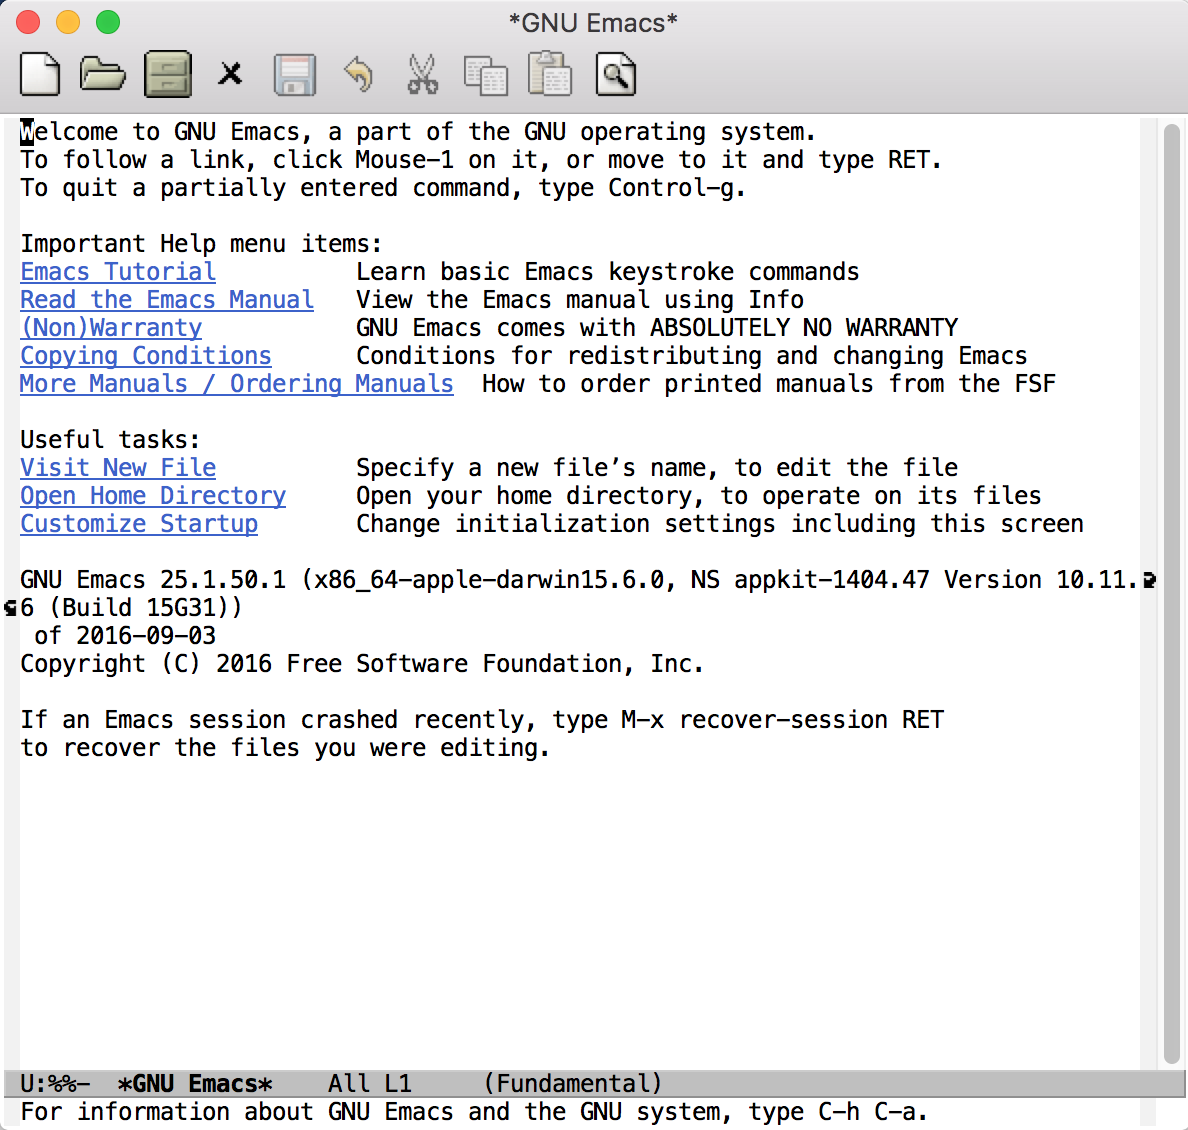
\includegraphics{figures/emacs.png}
\caption{Emacs Scratch Window}
\end{figure}

    \subsection{Python}\label{python}

\subsubsection{Introduction}\label{introduction}

Python is a programming language which is used and documented
extensively by the scientific communtiy. We use python to interface and
understand the Atomic Simulation Environment (ASE) which is used to
build, setup and modify molecular models. The best resources for
learning scientific python is through
\href{http://www.scipy-lectures.org/}{SciPy} which has extensive notes
and examples on using python for scientific computing.
\href{http://kitchingroup.cheme.cmu.edu/pycse/pycse.html}{PYCSE} is a
module written by \href{http://kitchingroup.cheme.cmu.edu/}{John
Kitchin} and has many examples which use standard Python Modules as well
as custom modules in PYCSE. We recommend that you practice these
examples as much as possible to obtain a good understanding of python
and how to use it to suit your needs.

    \subsubsection{Getting in the Groove}\label{getting-in-the-groove}

This section shows some of the more common commands and functions that
you will see in python scripts used by some of the group members. Again,
we encourage you to review the massive/huge documentation for
\href{https://docs.python.org/2/}{python}

On a command line, the python interpreter can be accessed through the
command \texttt{python} assuming that python is installed in it. The
following code blocks will be executable if you are using the iPython
Notebook. If you are using the read-only html or pdf versions of the
tutorial, you can copy the python code onto the interpreter, or onto a
script.

    \paragraph{Print}\label{print}

The simplest and most common bit of code ever created!

    \begin{Verbatim}[commandchars=\\\{\}]
{\color{incolor}In [{\color{incolor}1}]:} \PY{k}{print} \PY{l+s+s1}{\PYZsq{}}\PY{l+s+s1}{Hello, this is a sample sentence!}\PY{l+s+s1}{\PYZsq{}}
        \PY{k}{print} \PY{l+s+s1}{\PYZsq{}}\PY{l+s+s1}{This}\PY{l+s+se}{\PYZbs{}t}\PY{l+s+s1}{is}\PY{l+s+se}{\PYZbs{}t}\PY{l+s+s1}{tab}\PY{l+s+se}{\PYZbs{}t}\PY{l+s+s1}{separated}\PY{l+s+se}{\PYZbs{}t}\PY{l+s+s1}{text}\PY{l+s+s1}{\PYZsq{}}
\end{Verbatim}


    \begin{Verbatim}[commandchars=\\\{\}]
Hello, this is a sample sentence!
This	is	tab	separated	text

    \end{Verbatim}

    \paragraph{Arrays and Dictionaries}\label{arrays-and-dictionaries}

Arrays and dictionaries are useful data types used to store large
amounts of data that can be easily accessed and indexed. They can become
fairly complex, but the following code block shows a simple application
of these data types. We suggest that the reader builds a working
knowledge of these data types, given the data-intensive nature of the
work done in the group.

Numpy arrays and lists are interchangeable datatypes that behave
differently. Numpy is an immensely powerful python module with built-in
functionalitites that take care of most commonly mathematical
operations. The type of array that Numpy generates is called an
\texttt{numpy.ndarray}.

Dictionaries are data structures that work on the concept of key-value
pairs, where the key is used to index the dictionary and extract the
value corresponding to the key. Much like 2D and 3D arrays, dictionaries
can be nested within themselves to create massive data-structures and
databases.

    \begin{Verbatim}[commandchars=\\\{\}]
{\color{incolor}In [{\color{incolor}3}]:} \PY{k+kn}{import} \PY{n+nn}{numpy} \PY{k+kn}{as} \PY{n+nn}{np}
        
        \PY{c+c1}{\PYZsh{} Array with a range of numbers from 0 to 5, with step size of 1.}
        \PY{c+c1}{\PYZsh{} Here, the end point is not included.}
        \PY{n}{a} \PY{o}{=} \PY{n}{np}\PY{o}{.}\PY{n}{arange}\PY{p}{(}\PY{l+m+mi}{0}\PY{p}{,} \PY{l+m+mi}{5}\PY{p}{,} \PY{l+m+mi}{1}\PY{p}{)}
        \PY{k}{print} \PY{n}{a}
        
        \PY{c+c1}{\PYZsh{} Array with 10 numbers between 0 and 1}
        \PY{n}{a} \PY{o}{=} \PY{n}{np}\PY{o}{.}\PY{n}{linspace}\PY{p}{(}\PY{l+m+mi}{0}\PY{p}{,} \PY{l+m+mi}{5}\PY{p}{,} \PY{l+m+mi}{10}\PY{p}{)}
        \PY{k}{print} \PY{n}{a}
        
        \PY{c+c1}{\PYZsh{} Dictionary with keys and corresponding values showing date format}
        \PY{n}{b} \PY{o}{=} \PY{p}{\PYZob{}}\PY{l+s+s1}{\PYZsq{}}\PY{l+s+s1}{Day}\PY{l+s+s1}{\PYZsq{}}\PY{p}{:} \PY{l+s+s1}{\PYZsq{}}\PY{l+s+s1}{DD}\PY{l+s+s1}{\PYZsq{}}\PY{p}{,}
             \PY{l+s+s1}{\PYZsq{}}\PY{l+s+s1}{Month}\PY{l+s+s1}{\PYZsq{}}\PY{p}{:} \PY{l+s+s1}{\PYZsq{}}\PY{l+s+s1}{MM}\PY{l+s+s1}{\PYZsq{}}\PY{p}{,}
             \PY{l+s+s1}{\PYZsq{}}\PY{l+s+s1}{Year}\PY{l+s+s1}{\PYZsq{}}\PY{p}{:} \PY{l+s+s1}{\PYZsq{}}\PY{l+s+s1}{YYYY}\PY{l+s+s1}{\PYZsq{}}\PY{p}{\PYZcb{}}
        
        \PY{k}{print} \PY{n}{b}
        \PY{k}{print} \PY{n}{b}\PY{p}{[}\PY{l+s+s1}{\PYZsq{}}\PY{l+s+s1}{Month}\PY{l+s+s1}{\PYZsq{}}\PY{p}{]}
\end{Verbatim}


    \begin{Verbatim}[commandchars=\\\{\}]
[0 1 2 3 4]
[0.         0.55555556 1.11111111 1.66666667 2.22222222 2.77777778
 3.33333333 3.88888889 4.44444444 5.        ]
\{'Year': 'YYYY', 'Day': 'DD', 'Month': 'MM'\}
MM

    \end{Verbatim}

    \paragraph{Types of Variables}\label{types-of-variables}

Here we will define 4 types of variables: string variables, scalar
variables (either integer or float numbers), vector or 1-D array and
matrix or 2-D array.

    \begin{Verbatim}[commandchars=\\\{\}]
{\color{incolor}In [{\color{incolor}5}]:} \PY{n}{string} \PY{o}{=} \PY{l+s+s1}{\PYZsq{}}\PY{l+s+s1}{sample text}\PY{l+s+s1}{\PYZsq{}}
        \PY{n}{scalar} \PY{o}{=} \PY{l+m+mi}{12}
        \PY{n}{array\PYZus{}1d} \PY{o}{=} \PY{p}{[}\PY{l+m+mi}{1}\PY{p}{,}\PY{l+m+mi}{3}\PY{p}{,}\PY{l+m+mi}{6}\PY{p}{,}\PY{o}{\PYZhy{}}\PY{l+m+mi}{4}\PY{p}{,}\PY{l+m+mf}{0.95}\PY{p}{]}
        \PY{n}{array\PYZus{}2d} \PY{o}{=} \PY{p}{[}\PY{p}{[}\PY{l+m+mi}{1}\PY{p}{,}\PY{l+m+mi}{2}\PY{p}{]}\PY{p}{,}\PY{p}{[}\PY{o}{\PYZhy{}}\PY{l+m+mi}{3}\PY{p}{,}\PY{l+m+mf}{2.0}\PY{p}{]}\PY{p}{]}
        
        \PY{k}{print} \PY{n}{string} 
        \PY{k}{print} \PY{n}{scalar}
        \PY{k}{print} \PY{n}{array\PYZus{}1d}
        \PY{k}{print} \PY{n}{array\PYZus{}2d}
\end{Verbatim}


    \begin{Verbatim}[commandchars=\\\{\}]
sample text
12
[1, 3, 6, -4, 0.95]
[[1, 2], [-3, 2.0]]

    \end{Verbatim}

    \subsubsection{Loading python modules and
functions}\label{loading-python-modules-and-functions}

To use the wonderful functionalities of python modules like
\texttt{numpy,\ scipy,\ matplotlib,\ pandas,\ ase} in addition to the
default modules the user must explicitly import them in the python
codes.

Probably the most common modules that you are going to use are these:

\begin{longtable}[]{@{}ccc@{}}
\toprule
Module & Example Functions & Description\tabularnewline
\midrule
\endhead
os & mkdir, makedirs chdir, getcwd, listdir path, symlink & System
I/O\tabularnewline
ase & Atom, Atoms, build & Create atoms objects\tabularnewline
ase.io & read, write & Atoms objects read and write\tabularnewline
ase.calculators & Vasp, NWChem & Setup and run
calculations\tabularnewline
shutil & copy, move & High level file I/O\tabularnewline
\bottomrule
\end{longtable}

Modules are loaded as follows. Module errors show up in the following
way.

    \begin{Verbatim}[commandchars=\\\{\}]
{\color{incolor}In [{\color{incolor}3}]:} \PY{c+c1}{\PYZsh{} import os}
        \PY{k+kn}{import} \PY{n+nn}{osa} \PY{c+c1}{\PYZsh{}typo}
        \PY{k+kn}{from} \PY{n+nn}{ase} \PY{k+kn}{import} \PY{n}{atoms}
        \PY{k+kn}{from} \PY{n+nn}{ase.io} \PY{k+kn}{import} \PY{n}{read}
        \PY{k+kn}{from} \PY{n+nn}{ase.calculators.vasp} \PY{k+kn}{import} \PY{n}{Vasp}
\end{Verbatim}


    \begin{Verbatim}[commandchars=\\\{\}]

        ---------------------------------------------------------------------------

        ImportError                               Traceback (most recent call last)

        <ipython-input-3-12e1b204f232> in <module>()
          1 \# import os
    ----> 2 import osa \#typo
          3 from ase import atoms
          4 from ase.io import read
          5 from ase.calculators.vasp import Vasp


        ImportError: No module named osa

    \end{Verbatim}

    \subsubsection{Simple data manipulation}\label{simple-data-manipulation}

Data extraction and manipulation is important when dealing with huge
data files or when automation is required in order to post-process the
data in an efficient way.

As an example, you want to determine the value of the lattice parameter
of a bulk structure that minimizes the energy of the system. A simple
approach to determine this value is to determine the energy of the
system while changing the the lattice constant. Then, the energy and
volume for each lattice constant is fit to an equation to obtain the
volume that minimizes the energy. From the volume, one can extract the
lattice constant given a shape of unit cell.

We will use python to extract data and manipulate them to create a
simple plot. Create a text file using \emph{vi} called py\_ex\_data.txt
and copy all lines. Note that data columns are separated by tabs.
\texttt{3.8\ -12.28653631\ 3.85\ \ \ \ -12.65124072\ 3.9\ -12.88611724\ 3.95\ \ \ \ -13.01158939\ 4\ \ \ -13.04446413\ 4.05\ \ \ \ -12.99864981\ 4.1\ -12.88660177\ 4.15\ \ \ \ -12.71939621\ 4.2\ -12.5064955}

    Therefore, executing the command

\texttt{cat\ \textgreater{}\ \ py\_ex\_data.txt\ \textless{}\textless{}\ EOF}
gives us

\begin{verbatim}
3.8 -12.28653631
3.85    -12.65124072
3.9 -12.88611724
3.95    -13.01158939
4   -13.04446413
4.05    -12.99864981
4.1 -12.88660177
4.15    -12.71939621
4.2 -12.5064955
EOF
\end{verbatim}

    A simple code to read this file and extract the datapoints could look
like the following:

    \begin{Verbatim}[commandchars=\\\{\}]
{\color{incolor}In [{\color{incolor}5}]:} \PY{k+kn}{import} \PY{n+nn}{matplotlib.pyplot} \PY{k+kn}{as} \PY{n+nn}{plt}
        
        \PY{c+c1}{\PYZsh{} This is a comment. }
        \PY{c+c1}{\PYZsh{} Reading data file.}
        \PY{n}{data} \PY{o}{=} \PY{n+nb}{open}\PY{p}{(}\PY{l+s+s1}{\PYZsq{}}\PY{l+s+s1}{py\PYZus{}ex\PYZus{}data.txt}\PY{l+s+s1}{\PYZsq{}}\PY{p}{,}\PY{l+s+s1}{\PYZsq{}}\PY{l+s+s1}{r}\PY{l+s+s1}{\PYZsq{}}\PY{p}{)}
        \PY{n}{lines} \PY{o}{=} \PY{n}{data}\PY{o}{.}\PY{n}{readlines}\PY{p}{(}\PY{p}{)}
        \PY{n}{a} \PY{o}{=} \PY{p}{[}\PY{p}{]}
        \PY{n}{e} \PY{o}{=} \PY{p}{[}\PY{p}{]}
        
        \PY{c+c1}{\PYZsh{} To go through all lines we conveniently use a FOR loop}
        \PY{c+c1}{\PYZsh{} All data is stored in the empty lists a and e}
        \PY{k}{for} \PY{n}{line} \PY{o+ow}{in} \PY{n}{lines}\PY{p}{:}
          \PY{n}{values} \PY{o}{=} \PY{n}{line}\PY{o}{.}\PY{n}{split}\PY{p}{(}\PY{p}{)}
          \PY{n}{a}\PY{o}{.}\PY{n}{append}\PY{p}{(}\PY{n}{values}\PY{p}{[}\PY{l+m+mi}{0}\PY{p}{]}\PY{p}{)}
          \PY{n}{e}\PY{o}{.}\PY{n}{append}\PY{p}{(}\PY{n}{values}\PY{p}{[}\PY{l+m+mi}{1}\PY{p}{]}\PY{p}{)}
        
        \PY{k}{print} \PY{n}{a}
        \PY{k}{print} \PY{n}{e}
        \PY{n}{plt}\PY{o}{.}\PY{n}{plot}\PY{p}{(}\PY{n}{a}\PY{p}{,}\PY{n}{e}\PY{p}{,}\PY{l+s+s1}{\PYZsq{}}\PY{l+s+s1}{s:k}\PY{l+s+s1}{\PYZsq{}}\PY{p}{)}
\end{Verbatim}


    \begin{Verbatim}[commandchars=\\\{\}]
['3.8', '3.85', '3.9', '3.95', '4', '4.05', '4.1', '4.15', '4.2']
['-12.28653631', '-12.65124072', '-12.88611724', '-13.01158939', '-13.04446413', '-12.99864981', '-12.88660177', '-12.71939621', '-12.5064955']

    \end{Verbatim}

\begin{Verbatim}[commandchars=\\\{\}]
{\color{outcolor}Out[{\color{outcolor}5}]:} [<matplotlib.lines.Line2D at 0x60fda3810>]
\end{Verbatim}
            
    \begin{center}
    \adjustimage{max size={0.9\linewidth}{0.9\paperheight}}{output_36_2.png}
    \end{center}
    { \hspace*{\fill} \\}
    
    \subsection{Atomic Simulation Environment
(ASE)}\label{atomic-simulation-environment-ase}

ASE is an Atomic Simulation Environment written in the Python
programming language with the aim of setting up, steering, and analyzing
atomistic simulations (adapted from
\href{https://wiki.fysik.dtu.dk/ase/about.html}{ASE}). The ASE has been
constructed with a number of ``design goals'' that make it:

\begin{itemize}
\item
  Easy to use: Setting up an atomistic total energy calculation or
  molecular dynamics simulation with ASE is simple and straightforward.
  ASE can be used via a graphical user interface, Command line tools and
  the Python language. Python scripts are easy to follow (see What is
  Python? for a short introduction). It is simple for new users to get
  access to all of the functionality of ASE.
\item
  Flexible: Since ASE is based on the Python scripting language it is
  possible to perform very complicated simulation tasks without any code
  modifications. For example, a sequence of calculations may be
  performed with the use of simple ``for-loop'' constructions. There
  exist ASE modules for performing many standard simulation tasks.
\item
  Customizable: The Python code in ASE is structured in modules intended
  for different purposes. There are ase.calculators for calculating
  energies, forces and stresses, ase.md and ase.optimize modules for
  controlling the motion of atoms, constraints objects and filters for
  performing nudged-elastic-band calculations etc. The modularity of the
  object-oriented code make it simple to contribute new functionality to
  ASE.
\item
  Pythonic: It fits nicely into the rest of the Python world with use of
  the popular NumPy package for numerical work (see Numeric arrays in
  Python for a short introduction). The use of the Python language
  allows ASE to be used both interactively as well as in scripts.
\end{itemize}

\subsubsection{Installing ASE}\label{installing-ase}

ASE is a bundle of python modules which can be invoked or loaded when
atomic simulations are required to be set up or analyzed. The easiest
way of installing ase, is to download the latest source tar ball from
the website. Once downloaded, the tar ball must be extracted, and
installation can be completed by running

\begin{verbatim}
python setup.py install --user
\end{verbatim}

Tt is necessary to add the installation path in your \emph{=.cshrc=}
file and add \textasciitilde{}/.local/bin to the front of your PATH
environment variable. This is dependent on the system you are using.
Adding this location onto your \texttt{\$PATH} environment variable
enables you to access \texttt{ase-gui} and \texttt{ase-db} from any
location on the system.

    \subsubsection{Reading and Viewing simple atoms
files}\label{reading-and-viewing-simple-atoms-files}

We have downloaded a standard \emph{cif} file (Crystallographic
Information Format) from the International Zeolite Website
\href{http://www.iza-online.org/}{IZA} as an example structure. The
\emph{cif} file is present as MFI.cif in this folder. The ASE module
\texttt{ase.io} has the functions read and write which are capable of
handling various formats for atomic structure, and can be used to set up
every forseeable future \textbf{Vasp} calculation. An example of how to
read a \emph{cif} file is shown in the code block below.

Alternately, you can are use the \texttt{ase.build} class to create
simple pre-defined gas-phase molecules. In this example, we will create
a \(H_2O\) molecule.

    \begin{Verbatim}[commandchars=\\\{\}]
{\color{incolor}In [{\color{incolor}15}]:} \PY{c+c1}{\PYZsh{} Import the read and write functions from the ase.io module.}
         \PY{k+kn}{from} \PY{n+nn}{ase.io} \PY{k+kn}{import} \PY{n}{read}\PY{p}{,} \PY{n}{write}
         
         \PY{c+c1}{\PYZsh{} Import the molecule function from ase.build}
         \PY{k+kn}{from} \PY{n+nn}{ase.build} \PY{k+kn}{import} \PY{n}{molecule}
         
         \PY{c+c1}{\PYZsh{} Import the visualize function to view the imported atoms object.}
         \PY{k+kn}{from} \PY{n+nn}{ase.visualize} \PY{k+kn}{import} \PY{n}{view}
         
         \PY{c+c1}{\PYZsh{} Load the cif file into a pythonic object called \PYZsq{}atoms\PYZsq{}.}
         \PY{c+c1}{\PYZsh{}atoms = read(\PYZsq{}MFI.cif\PYZsq{})}
         
         \PY{c+c1}{\PYZsh{} Load a water molecule from ase.build}
         \PY{n}{atoms} \PY{o}{=} \PY{n}{molecule}\PY{p}{(}\PY{l+s+s1}{\PYZsq{}}\PY{l+s+s1}{H2O}\PY{l+s+s1}{\PYZsq{}}\PY{p}{)}
         
         \PY{c+c1}{\PYZsh{} View the \PYZsq{}atoms\PYZsq{} object.}
         \PY{n}{view}\PY{p}{(}\PY{n}{atoms}\PY{p}{)}
\end{Verbatim}


    \textbf{Vasp} calculations require a certain set of input files for
calculation initialization. The file that consists of the initial
structure and cartesian coordinates of the model under investigation is
the \textbf{POSCAR}. One can simply read a \emph{cif} and write out a
\textbf{POSCAR} using the functions provided by the \texttt{ase.io}
module. An example of writing files of various formats is shown below

    \begin{Verbatim}[commandchars=\\\{\}]
{\color{incolor}In [{\color{incolor}7}]:} \PY{k+kn}{from} \PY{n+nn}{ase.io} \PY{k+kn}{import} \PY{n}{read}\PY{p}{,} \PY{n}{write}
        
        \PY{n}{atoms} \PY{o}{=} \PY{n}{read}\PY{p}{(}\PY{l+s+s1}{\PYZsq{}}\PY{l+s+s1}{MFI.cif}\PY{l+s+s1}{\PYZsq{}}\PY{p}{)}
        
        \PY{c+c1}{\PYZsh{} Write the cartesian coordinates file in the =vasp= POSCAR format.}
        \PY{c+c1}{\PYZsh{} File written in the folder \PYZsq{}images\PYZsq{}}
        \PY{n}{write}\PY{p}{(}\PY{l+s+s1}{\PYZsq{}}\PY{l+s+s1}{figures/POSCAR\PYZus{}ZSM\PYZhy{}5}\PY{l+s+s1}{\PYZsq{}}\PY{p}{,} \PY{n}{atoms}\PY{p}{)}
        
        \PY{c+c1}{\PYZsh{} Write the cartesian coordinates file in the =xyz= format}
        \PY{n}{write}\PY{p}{(}\PY{l+s+s1}{\PYZsq{}}\PY{l+s+s1}{figures/atoms.xyz}\PY{l+s+s1}{\PYZsq{}}\PY{p}{,} \PY{n}{atoms}\PY{p}{)}
\end{Verbatim}


    \subsubsection{Building gas phase
molecules}\label{building-gas-phase-molecules}

Smaller models involving gas phase molecules and simple surfaces are
usually built up from scratch, using the modules and functions availble
in \texttt{ase}. This can either be done through scripting or through
the \texttt{ase-gui} interface. Extensive documentation on using the
\texttt{ase-gui} can be accessed in the ASE
\href{https://wiki.fysik.dtu.dk/ase/ase/gui/gui.html}{documentation}.
Here, we will provide a quick introduction on creating different
systems.

The most simple demonstration to begin with would be to model a simple
gas phase molecule such as \(H_{2}O\). ASE provides a number of ways to
build and modify models, and we will explore two ways. 1) using python
scripting and 2) using the ASE Graphical user interface
\texttt{ase-gui}. We recommend that you use scripting wherever possible
as this keeps track of all changes made to the model including the
documentation.

Gas phase models are the simplest models to create and are the least
expensive in terms of computational processing requirements. Such
systems require that they are enclosed in a vacuum cell of certain
dimensions that depends on the dimensions of the model itself. The
presence of this cell ensures that when DFT calculations are performed
and periodic boundary conditions are implemented in \(x\), \(y\) and
\(z\) directions, there is minimal interaction between the neighboring
images. Hence, one should perform calculations to ensure that energies
and cell sizes are well converged, before proceeding to use data from
these calculations.

We will build a simple \(H_2O\) molecule in a box of 10 x 10 x 10
\(\AA\).

    \begin{Verbatim}[commandchars=\\\{\}]
{\color{incolor}In [{\color{incolor}12}]:} \PY{k+kn}{from} \PY{n+nn}{ase.build} \PY{k+kn}{import} \PY{n}{molecule}
         \PY{k+kn}{from} \PY{n+nn}{ase.visualize} \PY{k+kn}{import} \PY{n}{view}
         \PY{k+kn}{from} \PY{n+nn}{ase.io} \PY{k+kn}{import} \PY{n}{write}
         
         \PY{n}{atoms} \PY{o}{=} \PY{n}{molecule}\PY{p}{(}\PY{l+s+s1}{\PYZsq{}}\PY{l+s+s1}{H2O}\PY{l+s+s1}{\PYZsq{}}\PY{p}{)}
         \PY{n}{atoms}\PY{o}{.}\PY{n}{set\PYZus{}cell}\PY{p}{(}\PY{p}{[}\PY{l+m+mi}{10}\PY{p}{,} \PY{l+m+mi}{10}\PY{p}{,} \PY{l+m+mi}{10}\PY{p}{]}\PY{p}{)}
         \PY{n}{atoms}\PY{o}{.}\PY{n}{center}\PY{p}{(}\PY{p}{)}
         
         \PY{n}{write}\PY{p}{(}\PY{l+s+s1}{\PYZsq{}}\PY{l+s+s1}{figures/molec\PYZus{}h2o\PYZus{}ase\PYZus{}ex.png}\PY{l+s+s1}{\PYZsq{}}\PY{p}{,} \PY{n}{atoms}\PY{p}{)}
         
         \PY{n}{view}\PY{p}{(}\PY{n}{atoms}\PY{p}{)}
\end{Verbatim}


    \begin{figure}
\centering
\includegraphics{figures/molec_h2o_ase_ex.png}
\caption{H2O Molecule}
\end{figure}

As you can see we have used the \texttt{molecule} and \texttt{view}
functions from the \texttt{ase.build} and \texttt{ase.visualize} modules
to build and visualize the molecule. Again, you need to load
installed/non-default python packages to use them in code.

The next example looks at building a model, or an \texttt{atoms} object
by explicity setting the element, its cartesian coordinates and the cell
size of the structure through code.

    \begin{Verbatim}[commandchars=\\\{\}]
{\color{incolor}In [{\color{incolor}15}]:} \PY{c+c1}{\PYZsh{} Import the Atoms and Atom modules}
         \PY{k+kn}{from} \PY{n+nn}{ase} \PY{k+kn}{import} \PY{n}{Atom}\PY{p}{,} \PY{n}{Atoms}
         \PY{k+kn}{from} \PY{n+nn}{ase.visualize} \PY{k+kn}{import} \PY{n}{view}
         \PY{k+kn}{from} \PY{n+nn}{ase.io} \PY{k+kn}{import} \PY{n}{read}\PY{p}{,} \PY{n}{write}
         
         \PY{c+c1}{\PYZsh{} Creating a random model with H, O and C at random positions}
         \PY{n}{atoms} \PY{o}{=} \PY{n}{Atoms}\PY{p}{(}\PY{p}{[}\PY{n}{Atom}\PY{p}{(}\PY{l+s+s1}{\PYZsq{}}\PY{l+s+s1}{H}\PY{l+s+s1}{\PYZsq{}}\PY{p}{,} \PY{p}{[}\PY{l+m+mi}{0}\PY{p}{,} \PY{l+m+mi}{0}\PY{p}{,} \PY{l+m+mi}{0}\PY{p}{]}\PY{p}{)}\PY{p}{,}
                        \PY{n}{Atom}\PY{p}{(}\PY{l+s+s1}{\PYZsq{}}\PY{l+s+s1}{O}\PY{l+s+s1}{\PYZsq{}}\PY{p}{,} \PY{p}{[}\PY{l+m+mi}{1}\PY{p}{,} \PY{l+m+mi}{1}\PY{p}{,} \PY{l+m+mi}{1}\PY{p}{]}\PY{p}{)}\PY{p}{,} 
                        \PY{n}{Atom}\PY{p}{(}\PY{l+s+s1}{\PYZsq{}}\PY{l+s+s1}{C}\PY{l+s+s1}{\PYZsq{}}\PY{p}{,} \PY{p}{[}\PY{l+m+mi}{2}\PY{p}{,} \PY{l+m+mi}{2}\PY{p}{,} \PY{l+m+mi}{1}\PY{p}{]}\PY{p}{)}\PY{p}{]}\PY{p}{)}
         
         \PY{c+c1}{\PYZsh{} Set a cell of dimensions 10 \PYZbs{}AA}
         \PY{n}{atoms}\PY{o}{.}\PY{n}{set\PYZus{}cell}\PY{p}{(}\PY{p}{[}\PY{l+m+mi}{10}\PY{p}{,} \PY{l+m+mi}{10}\PY{p}{,} \PY{l+m+mi}{10}\PY{p}{]}\PY{p}{)}
         \PY{n}{write}\PY{p}{(}\PY{l+s+s1}{\PYZsq{}}\PY{l+s+s1}{figures/not\PYZhy{}centered.png}\PY{l+s+s1}{\PYZsq{}}\PY{p}{,} \PY{n}{atoms}\PY{p}{,} \PY{n}{show\PYZus{}unit\PYZus{}cell}\PY{o}{=}\PY{n+nb+bp}{True}\PY{p}{)}
         \PY{c+c1}{\PYZsh{} The atoms and the cell originate at [0, 0, 0], and the model will not be centered within the cell}
         \PY{c+c1}{\PYZsh{} it is important to center the model so that there is equal vacuum on all sides.}
         \PY{n}{atoms}\PY{o}{.}\PY{n}{center}\PY{p}{(}\PY{p}{)}
         
         \PY{n}{write}\PY{p}{(}\PY{l+s+s1}{\PYZsq{}}\PY{l+s+s1}{figures/centered.png}\PY{l+s+s1}{\PYZsq{}}\PY{p}{,} \PY{n}{atoms}\PY{p}{,} \PY{n}{show\PYZus{}unit\PYZus{}cell}\PY{o}{=}\PY{n+nb+bp}{True}\PY{p}{)}
         \PY{n}{write}\PY{p}{(}\PY{l+s+s1}{\PYZsq{}}\PY{l+s+s1}{figures/POSCAR\PYZus{}random}\PY{l+s+s1}{\PYZsq{}}\PY{p}{,} \PY{n}{atoms}\PY{p}{,} \PY{n}{format}\PY{o}{=}\PY{l+s+s1}{\PYZsq{}}\PY{l+s+s1}{vasp}\PY{l+s+s1}{\PYZsq{}}\PY{p}{)}
\end{Verbatim}


    \includegraphics{figures/not-centered.png}
\includegraphics{figures/centered.png}

    \paragraph{Building crystal
structures}\label{building-crystal-structures}

Crystals are isotropic materials that maintain an order in a microscopic
scale and in all three dimensions. The building block or the unit cell
in a crystal when repeated many times in all directions creates a
macroscopic form of the crystal. In computational simulations, reactions
that take place over catalysts are typicall simulated over moldes that
contain a small number of unit cells, with the assumption that the
thermodynamics and kinetics at the microscopic scale is reproducible at
the macroscopic sclae. The example in the following figure is the
structure of the rutile-phase of \(TiO_{2}\). In this figure, the
dashed-line box represent the limits of the unit cell that is repeated
in all directions.

\href{figures/rut-TiO2.png}{Unit cell of Rutile TiO2}

This structure can be created with ASE by using the
\texttt{ase.spacegroup} module. The create function requires that you to
provide the crystal spacegroup, the lattice parameters and the scaled
positions of the unique atoms (the number of atoms provided not
necessarily match with the number of atoms in the unit cell). We will
need detailed information about \(TiO_2\) which can be found in
scientific articles or databases such as
\href{materialsproject.org}{Materials Project}. A python script that
creates a rutile \(TiO_2\) bulk crystal is given below

    \begin{Verbatim}[commandchars=\\\{\}]
{\color{incolor}In [{\color{incolor}17}]:} \PY{k+kn}{from} \PY{n+nn}{ase.lattice.spacegroup} \PY{k+kn}{import} \PY{n}{crystal}
         \PY{k+kn}{from} \PY{n+nn}{ase.visualize} \PY{k+kn}{import} \PY{n}{view}
         \PY{k+kn}{from} \PY{n+nn}{ase.io} \PY{k+kn}{import} \PY{n}{write}
         
         \PY{c+c1}{\PYZsh{} Lattice parameters. Experimetnal values for TiO2 rutile}
         \PY{n}{a} \PY{o}{=} \PY{l+m+mf}{4.5937}
         \PY{n}{c} \PY{o}{=} \PY{l+m+mf}{2.9587}
         
         \PY{c+c1}{\PYZsh{} Using the \PYZsq{}crystal\PYZsq{} function from \PYZsq{}spacegroup\PYZsq{} subpackage}
         \PY{c+c1}{\PYZsh{} Data provided (in order of appearence)}
         \PY{c+c1}{\PYZsh{} Unique atoms in unit cell; scaled positions of unique atoms;}
         \PY{c+c1}{\PYZsh{} Space group ID \PYZsh{}; dimension of unit cell (lattice param. and angles)}
         \PY{n}{rut} \PY{o}{=} \PY{n}{crystal}\PY{p}{(}\PY{p}{[}\PY{l+s+s1}{\PYZsq{}}\PY{l+s+s1}{Ti}\PY{l+s+s1}{\PYZsq{}}\PY{p}{,}\PY{l+s+s1}{\PYZsq{}}\PY{l+s+s1}{O}\PY{l+s+s1}{\PYZsq{}}\PY{p}{]}\PY{p}{,} \PY{n}{basis}\PY{o}{=}\PY{p}{[}\PY{p}{(}\PY{l+m+mf}{0.0}\PY{p}{,}\PY{l+m+mf}{0.0}\PY{p}{,}\PY{l+m+mf}{0.0}\PY{p}{)}\PY{p}{,}\PY{p}{(}\PY{l+m+mf}{0.3048}\PY{p}{,}\PY{l+m+mf}{0.3048}\PY{p}{,}\PY{l+m+mf}{0.0}\PY{p}{)}\PY{p}{]}\PY{p}{,}
            \PY{n}{spacegroup}\PY{o}{=}\PY{l+m+mi}{136}\PY{p}{,} \PY{n}{cellpar}\PY{o}{=}\PY{p}{[}\PY{n}{a}\PY{p}{,} \PY{n}{a}\PY{p}{,} \PY{n}{c}\PY{p}{,} \PY{l+m+mi}{90}\PY{p}{,} \PY{l+m+mi}{90}\PY{p}{,} \PY{l+m+mi}{90}\PY{p}{]}\PY{p}{)}
         
         \PY{n}{write}\PY{p}{(}\PY{l+s+s1}{\PYZsq{}}\PY{l+s+s1}{figures/rut\PYZhy{}TiO2.png}\PY{l+s+s1}{\PYZsq{}}\PY{p}{,} \PY{n}{rut}\PY{p}{)}
         \PY{n}{view}\PY{p}{(}\PY{n}{rut}\PY{p}{)}
\end{Verbatim}


    The \texttt{ase-gui} windows that pops up shows the unit cell of
rut-TiO\_\{2\} and it consists of two Ti and four O atoms. However, we
only specified two coordinates(Ti and O) in the script. The
\texttt{spacegroup} argument lets \texttt{ASE} know where the other
equivalent atoms should be placed according to symmetric positions that
are dependent of the space group.

The unit cell information and the atomic positions are based on
experimental values. In almost all cases, these parameters have to be
optimized for the user defined computational settings (cutoffs,
accuracy, physics) before it can be used to generate a surface or for
actual potential energy surfaces. Bulk structure optimization will be
looked into at a later point in this tutorial.

    \paragraph{Building surfaces}\label{building-surfaces}

If you want to simulate the adsorption of a chemical species and its
interaction with a heterogeneous catalyst, you might want to create a
representative model of the surface/bulk model in question. Here, we
explain how one can create a surface model that could be used for
calculations such as adsorption.

We will build a slab of the (101) exposed facet of tetragonal zirconium
oxide \(ZrO_2\) from its crystal structure parameters. First, you will
need the lattice parameters required to build a bulk crystal (as was
done for \(rut-TiO_2\) above). The lattice parameters are shown in the
codeblock below, together with an extra line with the function
\texttt{surface} that can be used to build a surface from a bulk
crystal. In this case, the function needs an \texttt{atoms} object
(\texttt{atoms} in the code), the plane at which the cut should be
considered, the number of layers that should be included in the \(z\)
direction and the thickness of the vacuum layer in each side of slab (in
angstroms).

    \begin{Verbatim}[commandchars=\\\{\}]
{\color{incolor}In [{\color{incolor}19}]:} \PY{k+kn}{from} \PY{n+nn}{ase.lattice.spacegroup} \PY{k+kn}{import} \PY{n}{crystal}
         \PY{k+kn}{from} \PY{n+nn}{ase.visualize} \PY{k+kn}{import} \PY{n}{view}
         \PY{k+kn}{from} \PY{n+nn}{ase.lattice.surface} \PY{k+kn}{import} \PY{n}{surface}
         \PY{k+kn}{from} \PY{n+nn}{ase.io} \PY{k+kn}{import} \PY{n}{read}\PY{p}{,} \PY{n}{write}
         
         \PY{n}{a} \PY{o}{=} \PY{l+m+mf}{3.63}
         \PY{n}{c} \PY{o}{=} \PY{l+m+mf}{5.25}
         \PY{n}{z} \PY{o}{=} \PY{l+m+mf}{0.05}
         
         \PY{n}{atoms} \PY{o}{=} \PY{n}{crystal}\PY{p}{(}\PY{p}{[}\PY{l+s+s1}{\PYZsq{}}\PY{l+s+s1}{Zr}\PY{l+s+s1}{\PYZsq{}}\PY{p}{,} \PY{l+s+s1}{\PYZsq{}}\PY{l+s+s1}{O}\PY{l+s+s1}{\PYZsq{}}\PY{p}{]}\PY{p}{,} \PY{n}{basis}\PY{o}{=}\PY{p}{[}\PY{p}{(}\PY{l+m+mf}{0.0}\PY{p}{,} \PY{l+m+mf}{0.0}\PY{p}{,} \PY{l+m+mf}{0.0}\PY{p}{)}\PY{p}{,} \PY{p}{(}\PY{l+m+mf}{0.0}\PY{p}{,} \PY{l+m+mf}{0.5}\PY{p}{,} \PY{n}{z}\PY{o}{+}\PY{l+m+mf}{0.25}\PY{p}{)}\PY{p}{]}\PY{p}{,}
            \PY{n}{spacegroup}\PY{o}{=}\PY{l+m+mi}{137}\PY{p}{,} \PY{n}{cellpar}\PY{o}{=}\PY{p}{[}\PY{n}{a}\PY{p}{,} \PY{n}{a}\PY{p}{,} \PY{n}{c}\PY{p}{,} \PY{l+m+mi}{90}\PY{p}{,} \PY{l+m+mi}{90}\PY{p}{,} \PY{l+m+mi}{90}\PY{p}{]}\PY{p}{)}
         
         \PY{n}{surface} \PY{o}{=} \PY{n}{surface}\PY{p}{(}\PY{n}{atoms}\PY{p}{,} \PY{p}{(}\PY{l+m+mi}{1}\PY{p}{,}\PY{l+m+mi}{0}\PY{p}{,}\PY{l+m+mi}{1}\PY{p}{)}\PY{p}{,} \PY{l+m+mi}{5}\PY{p}{,} \PY{l+m+mf}{7.5}\PY{p}{)}
         
         \PY{n}{write}\PY{p}{(}\PY{l+s+s1}{\PYZsq{}}\PY{l+s+s1}{ZrO2\PYZus{}surf\PYZus{}ex.png}\PY{l+s+s1}{\PYZsq{}}\PY{p}{,} \PY{n}{surface}\PY{p}{)}
         \PY{n}{view}\PY{p}{(}\PY{n}{surface}\PY{p}{)}
\end{Verbatim}


    \href{figures/ZrO2_surf_ex.png}{ZrO2 Surface}

Even though this process is fairly simple, one needs to be careful in
the selection of the surface termination. For instance, by looking at
the slab generated by ASE one can see that the exposed surface in +z
direction has a oxygen termination, that might not be (and is not) the
most stable termination. However, by deleting "extra" oxygen atoms on
top, we are also changing the Zr/O ratio. The surface slab is now no
longer stoichiometric (\(Zr_{10}O_{18}\) instead of \(Zr_{10}O_{20}\).
There are multiple solutions to these problems and the best solution
depends on the case. This is usually not a problem for simple metal
surfaces that are highly symetrical and pure.

A simple solution to this problem can be creating a slab with an extra
layer and then deleting the atoms that are not longer needed in order to
maintain the desirable number of layers. At the end, is possible that we
need to shift the position of all atoms in the cell in order to keep the
center of mass in the center of the cell. We are going to use a similar
script to create a slab with an extra layer and then delete some of the
atoms, so we keep only 5 layers in total.

    \begin{Verbatim}[commandchars=\\\{\}]
{\color{incolor}In [{\color{incolor}20}]:} \PY{k+kn}{from} \PY{n+nn}{ase.lattice.spacegroup} \PY{k+kn}{import} \PY{n}{crystal}
         \PY{k+kn}{from} \PY{n+nn}{ase.visualize} \PY{k+kn}{import} \PY{n}{view}
         \PY{k+kn}{from} \PY{n+nn}{ase.lattice.surface} \PY{k+kn}{import} \PY{n}{surface}
         
         \PY{n}{a} \PY{o}{=} \PY{l+m+mf}{3.63}
         \PY{n}{c} \PY{o}{=} \PY{l+m+mf}{5.25}
         \PY{n}{z} \PY{o}{=} \PY{l+m+mf}{0.05}
         
         \PY{n}{atoms} \PY{o}{=} \PY{n}{crystal}\PY{p}{(}\PY{p}{[}\PY{l+s+s1}{\PYZsq{}}\PY{l+s+s1}{Zr}\PY{l+s+s1}{\PYZsq{}}\PY{p}{,} \PY{l+s+s1}{\PYZsq{}}\PY{l+s+s1}{O}\PY{l+s+s1}{\PYZsq{}}\PY{p}{]}\PY{p}{,} \PY{n}{basis}\PY{o}{=}\PY{p}{[}\PY{p}{(}\PY{l+m+mf}{0.0}\PY{p}{,} \PY{l+m+mf}{0.0}\PY{p}{,} \PY{l+m+mf}{0.0}\PY{p}{)}\PY{p}{,} \PY{p}{(}\PY{l+m+mf}{0.0}\PY{p}{,} \PY{l+m+mf}{0.5}\PY{p}{,} \PY{n}{z}\PY{o}{+}\PY{l+m+mf}{0.25}\PY{p}{)}\PY{p}{]}\PY{p}{,}
            \PY{n}{spacegroup}\PY{o}{=}\PY{l+m+mi}{137}\PY{p}{,} \PY{n}{cellpar}\PY{o}{=}\PY{p}{[}\PY{n}{a}\PY{p}{,} \PY{n}{a}\PY{p}{,} \PY{n}{c}\PY{p}{,} \PY{l+m+mi}{90}\PY{p}{,} \PY{l+m+mi}{90}\PY{p}{,} \PY{l+m+mi}{90}\PY{p}{]}\PY{p}{)}
         
         \PY{n}{surface} \PY{o}{=} \PY{n}{surface}\PY{p}{(}\PY{n}{atoms}\PY{p}{,} \PY{p}{(}\PY{l+m+mi}{1}\PY{p}{,}\PY{l+m+mi}{0}\PY{p}{,}\PY{l+m+mi}{1}\PY{p}{)}\PY{p}{,} \PY{l+m+mi}{6}\PY{p}{,} \PY{l+m+mf}{7.5}\PY{p}{)}
         
         \PY{c+c1}{\PYZsh{} Lets remove the atoms that should lead to a 5\PYZhy{}layered non\PYZhy{}oxygen terminated stoichiometric surface}
         \PY{n}{ind2remove} \PY{o}{=} \PY{p}{[}\PY{l+m+mi}{0}\PY{p}{,}\PY{l+m+mi}{1}\PY{p}{,}\PY{l+m+mi}{2}\PY{p}{,}\PY{l+m+mi}{5}\PY{p}{,}\PY{l+m+mi}{33}\PY{p}{,}\PY{l+m+mi}{34}\PY{p}{]}
         \PY{k}{for} \PY{n}{i} \PY{o+ow}{in} \PY{n+nb}{sorted}\PY{p}{(}\PY{n}{ind2remove}\PY{p}{,} \PY{n}{reverse}\PY{o}{=}\PY{n+nb+bp}{True}\PY{p}{)}\PY{p}{:}
            \PY{k}{del} \PY{n}{surface}\PY{p}{[}\PY{n}{i}\PY{p}{]}
         
         \PY{c+c1}{\PYZsh{} Translate atoms to the new center}
         \PY{n}{cell} \PY{o}{=} \PY{n}{surface}\PY{o}{.}\PY{n}{get\PYZus{}cell}\PY{p}{(}\PY{p}{)}
         \PY{n}{com} \PY{o}{=} \PY{n}{surface}\PY{o}{.}\PY{n}{get\PYZus{}center\PYZus{}of\PYZus{}mass}\PY{p}{(}\PY{p}{)}
         \PY{n}{surface}\PY{o}{.}\PY{n}{translate}\PY{p}{(}\PY{p}{[}\PY{l+m+mi}{0}\PY{p}{,}\PY{l+m+mi}{0}\PY{p}{,}\PY{l+m+mf}{0.5}\PY{o}{*}\PY{n}{cell}\PY{p}{[}\PY{l+m+mi}{2}\PY{p}{,}\PY{l+m+mi}{2}\PY{p}{]} \PY{o}{\PYZhy{}} \PY{n}{com}\PY{p}{[}\PY{l+m+mi}{2}\PY{p}{]}\PY{p}{]}\PY{p}{)}
         
         \PY{n}{view}\PY{p}{(}\PY{n}{surface}\PY{p}{)}
\end{Verbatim}


    As a result, you should get a new slab with the right termination but
also one that keeps the Zr/O ratio to 1/2. In the script, we have
specified the indices of atoms that are to be deleted, then we shift the
position of the whole slab in the z-direction so the center of mass of
the slab resides again in the center of the cell.

    \subsubsection{Get details of an atoms
object}\label{get-details-of-an-atoms-object}

\texttt{ASE} has many useful functions which when used efficiently are
very powerful in automating scripts and workflow. Given that we have
already learned to build complex models and structures, we must also
know how to extract details from atoms objects, in the case of analysis
and post-processing. Examples of simple ase functions for this purpose
are shown below.

    \begin{Verbatim}[commandchars=\\\{\}]
{\color{incolor}In [{\color{incolor}21}]:} \PY{k+kn}{from} \PY{n+nn}{ase.io} \PY{k+kn}{import} \PY{n}{read}
         
         \PY{c+c1}{\PYZsh{} Read atoms from previously stored POSCAR}
         \PY{n}{atoms} \PY{o}{=} \PY{n}{read}\PY{p}{(}\PY{l+s+s1}{\PYZsq{}}\PY{l+s+s1}{figures/POSCAR\PYZus{}ZSM\PYZhy{}5}\PY{l+s+s1}{\PYZsq{}}\PY{p}{)}
         
         \PY{c+c1}{\PYZsh{} Get unit cell parameters}
         \PY{n}{cell} \PY{o}{=} \PY{n}{atoms}\PY{o}{.}\PY{n}{get\PYZus{}cell}\PY{p}{(}\PY{p}{)}
         \PY{k}{print} \PY{l+s+s1}{\PYZsq{}}\PY{l+s+s1}{Unit cell array:}\PY{l+s+s1}{\PYZsq{}} 
         \PY{k}{print} \PY{n}{cell}\PY{p}{,} \PY{l+s+s1}{\PYZsq{}}\PY{l+s+se}{\PYZbs{}n}\PY{l+s+s1}{\PYZsq{}}
         
         \PY{c+c1}{\PYZsh{} Get details of all individual atoms making up the entire atoms object}
         \PY{c+c1}{\PYZsh{} Printing only first 10 atom details, using python list indexing}
         \PY{k}{print}\PY{p}{(}\PY{l+s+s1}{\PYZsq{}}\PY{l+s+s1}{Details of 10 individual atoms: }\PY{l+s+s1}{\PYZsq{}}\PY{p}{)}
         \PY{k}{for} \PY{n}{atom} \PY{o+ow}{in} \PY{n}{atoms}\PY{p}{[}\PY{l+m+mi}{0}\PY{p}{:}\PY{l+m+mi}{10}\PY{p}{]}\PY{p}{:}
             \PY{k}{print} \PY{n}{atom}
         
         \PY{c+c1}{\PYZsh{} Get positions of atoms, and print specific details}
         \PY{n}{positions} \PY{o}{=} \PY{n}{atoms}\PY{o}{.}\PY{n}{get\PYZus{}positions}\PY{p}{(}\PY{p}{)}
         
         \PY{c+c1}{\PYZsh{} Using python string formatting and enumeration concepts}
         \PY{k}{print}\PY{p}{(}\PY{l+s+s1}{\PYZsq{}}\PY{l+s+se}{\PYZbs{}n}\PY{l+s+s1}{Atom specific details: }\PY{l+s+s1}{\PYZsq{}}\PY{p}{)}
         \PY{k}{for} \PY{n}{i}\PY{p}{,} \PY{n}{atom} \PY{o+ow}{in} \PY{n+nb}{enumerate}\PY{p}{(}\PY{n}{atoms}\PY{p}{[}\PY{l+m+mi}{0}\PY{p}{:}\PY{l+m+mi}{10}\PY{p}{]}\PY{p}{)}\PY{p}{:}
             \PY{k}{print}\PY{p}{(}\PY{l+s+s1}{\PYZsq{}}\PY{l+s+s1}{Index: \PYZob{}0\PYZcb{}, Element: \PYZob{}1\PYZcb{}, Coordinates: \PYZob{}2\PYZcb{}}\PY{l+s+s1}{\PYZsq{}}\PY{o}{.}\PY{n}{format}\PY{p}{(}\PY{n}{i}\PY{p}{,} \PY{n}{atom}\PY{o}{.}\PY{n}{symbol}\PY{p}{,} \PY{n}{positions}\PY{p}{[}\PY{n}{i}\PY{p}{]}\PY{p}{)}\PY{p}{)}
\end{Verbatim}


    \begin{Verbatim}[commandchars=\\\{\}]
Unit cell array:
[[20.09   0.     0.   ]
 [ 0.    19.738  0.   ]
 [ 0.     0.    13.142]] 

Details of 10 individual atoms: 
Atom('O', [10.069108, 1.3796862, 9.223055599999999], index=0)
Atom('O', [20.065892, 11.2486862, 2.6520555999999997], index=1)
Atom('O', [10.069108, 8.4893138, 9.223055599999999], index=2)
Atom('O', [20.065892, 18.3583138, 2.6520555999999997], index=3)
Atom('O', [10.020892, 18.3583138, 3.9189444], index=4)
Atom('O', [0.0241079999999973, 8.4893138, 10.4899444], index=5)
Atom('O', [10.020892, 11.2486862, 3.9189444], index=6)
Atom('O', [0.0241079999999973, 1.3796862, 10.4899444], index=7)
Atom('O', [7.784875, 1.4665334, 10.5241136], index=8)
Atom('O', [2.260125, 11.335533400000001, 3.953113599999999], index=9)

Atom specific details: 
Index: 0, Element: O, Coordinates: [10.069108   1.3796862  9.2230556]
Index: 1, Element: O, Coordinates: [20.065892  11.2486862  2.6520556]
Index: 2, Element: O, Coordinates: [10.069108   8.4893138  9.2230556]
Index: 3, Element: O, Coordinates: [20.065892  18.3583138  2.6520556]
Index: 4, Element: O, Coordinates: [10.020892  18.3583138  3.9189444]
Index: 5, Element: O, Coordinates: [ 0.024108   8.4893138 10.4899444]
Index: 6, Element: O, Coordinates: [10.020892  11.2486862  3.9189444]
Index: 7, Element: O, Coordinates: [ 0.024108   1.3796862 10.4899444]
Index: 8, Element: O, Coordinates: [ 7.784875   1.4665334 10.5241136]
Index: 9, Element: O, Coordinates: [ 2.260125  11.3355334  3.9531136]

    \end{Verbatim}

    \paragraph{Edit a loaded atoms object}\label{edit-a-loaded-atoms-object}

Pre-loaded structures loaded as \texttt{atoms} objects can be edited to
suit the requirements of the model and include other constraints. The
process of editing is simple. First, the relevant model
(\texttt{POSCAR,\ cif}, etc..) is loaded. Specific details like position
can be obtained using relevant functions. Modifications to these details
are then made, and finally, the modifications are implemented in the
atoms object using relevant functions. An example follows.

    \begin{Verbatim}[commandchars=\\\{\}]
{\color{incolor}In [{\color{incolor}22}]:} \PY{k+kn}{from} \PY{n+nn}{ase.io} \PY{k+kn}{import} \PY{n}{read}
         
         \PY{n}{atoms} \PY{o}{=} \PY{n}{read}\PY{p}{(}\PY{l+s+s1}{\PYZsq{}}\PY{l+s+s1}{figures/POSCAR\PYZus{}ZSM\PYZhy{}5}\PY{l+s+s1}{\PYZsq{}}\PY{p}{)}
         
         \PY{c+c1}{\PYZsh{} Store required atom into a new variable.}
         \PY{c+c1}{\PYZsh{} Note: This is usually done in less explicit ways}
         \PY{n}{atom} \PY{o}{=} \PY{n}{atoms}\PY{p}{[}\PY{l+m+mi}{4}\PY{p}{]}
         \PY{n}{positions} \PY{o}{=} \PY{n}{atoms}\PY{o}{.}\PY{n}{get\PYZus{}positions}\PY{p}{(}\PY{p}{)}
         
         \PY{c+c1}{\PYZsh{} Printing coordinates before implementing changes}
         \PY{k}{print} \PY{l+s+s1}{\PYZsq{}}\PY{l+s+s1}{Coordinates of atom number 4: }\PY{l+s+s1}{\PYZsq{}}\PY{p}{,} \PY{n}{atom}\PY{o}{.}\PY{n}{position}
         \PY{k}{print} \PY{l+s+s1}{\PYZsq{}}\PY{l+s+s1}{Element of atom number 4: }\PY{l+s+s1}{\PYZsq{}}\PY{p}{,} \PY{n}{atom}\PY{o}{.}\PY{n}{symbol}
         
         \PY{c+c1}{\PYZsh{} We want to change the element and cartesian coordinates of the atom with index=4.}
         \PY{n}{positions}\PY{p}{[}\PY{l+m+mi}{4}\PY{p}{]} \PY{o}{=} \PY{p}{[}\PY{l+m+mi}{1}\PY{p}{,} \PY{l+m+mi}{1}\PY{p}{,} \PY{l+m+mi}{1}\PY{p}{]}
         \PY{n}{atoms}\PY{p}{[}\PY{l+m+mi}{4}\PY{p}{]}\PY{o}{.}\PY{n}{symbol} \PY{o}{=} \PY{l+s+s1}{\PYZsq{}}\PY{l+s+s1}{C}\PY{l+s+s1}{\PYZsq{}}
         
         \PY{c+c1}{\PYZsh{} Reassign modified positions to original atoms object}
         \PY{n}{atoms}\PY{o}{.}\PY{n}{set\PYZus{}positions}\PY{p}{(}\PY{n}{positions}\PY{p}{)}
         
         \PY{k}{print} \PY{l+s+s1}{\PYZsq{}}\PY{l+s+se}{\PYZbs{}n}\PY{l+s+s1}{Details after implementing changes: }\PY{l+s+s1}{\PYZsq{}}
         \PY{n}{atom} \PY{o}{=} \PY{n}{atoms}\PY{p}{[}\PY{l+m+mi}{4}\PY{p}{]}
         \PY{k}{print} \PY{l+s+s1}{\PYZsq{}}\PY{l+s+s1}{Coordinates of atom number 4: }\PY{l+s+s1}{\PYZsq{}}\PY{p}{,} \PY{n}{atom}\PY{o}{.}\PY{n}{position}
         \PY{k}{print} \PY{l+s+s1}{\PYZsq{}}\PY{l+s+s1}{Element of atom number 4: }\PY{l+s+s1}{\PYZsq{}}\PY{p}{,} \PY{n}{atom}\PY{o}{.}\PY{n}{symbol}
\end{Verbatim}


    \begin{Verbatim}[commandchars=\\\{\}]
Coordinates of atom number 4:  [10.020892  18.3583138  3.9189444]
Element of atom number 4:  O

Details after implementing changes: 
Coordinates of atom number 4:  [1. 1. 1.]
Element of atom number 4:  C

    \end{Verbatim}

    \paragraph{Adding Atoms to Models}\label{adding-atoms-to-models}

The \texttt{atoms} object is essentially a \texttt{python} list of
individual atoms objects. Hence, one can perform the same operations on
atoms objects as simple lists. New atoms can be added to an existing
atoms object using the \texttt{append} function in python. However, if
you want to add an entire atoms object to a pre-existing atoms object,
then one must use python's \texttt{extend} function. Please do read up
the differences between \texttt{append()} and \texttt{extend()} for
clarity

In the example shown below, both atoms objects end up identical.

    \begin{Verbatim}[commandchars=\\\{\}]
{\color{incolor}In [{\color{incolor}23}]:} \PY{k+kn}{from} \PY{n+nn}{ase.io} \PY{k+kn}{import} \PY{n}{read}
         \PY{k+kn}{from} \PY{n+nn}{ase} \PY{k+kn}{import} \PY{n}{Atom}\PY{p}{,} \PY{n}{Atoms}
         
         \PY{c+c1}{\PYZsh{} Read in two pre\PYZhy{}existing atoms objects}
         \PY{n}{atoms} \PY{o}{=} \PY{n}{read}\PY{p}{(}\PY{l+s+s1}{\PYZsq{}}\PY{l+s+s1}{figures/POSCAR\PYZus{}ZSM\PYZhy{}5}\PY{l+s+s1}{\PYZsq{}}\PY{p}{)}
         \PY{n}{atoms\PYZus{}new} \PY{o}{=} \PY{n}{read}\PY{p}{(}\PY{l+s+s1}{\PYZsq{}}\PY{l+s+s1}{figures/POSCAR\PYZus{}random}\PY{l+s+s1}{\PYZsq{}}\PY{p}{)}
         
         \PY{c+c1}{\PYZsh{} Generate a copy of the original atoms object}
         \PY{n}{atoms1} \PY{o}{=} \PY{n}{atoms}\PY{o}{.}\PY{n}{copy}\PY{p}{(}\PY{p}{)}
         
         \PY{c+c1}{\PYZsh{} To add atoms\PYZus{}new to atoms, we use the extend() function}
         \PY{n}{atoms1}\PY{o}{.}\PY{n}{extend}\PY{p}{(}\PY{n}{atoms\PYZus{}new}\PY{p}{)}
         \PY{k}{print} \PY{n}{atoms1}
         
         \PY{c+c1}{\PYZsh{} Define explicit atom objects}
         \PY{n}{H} \PY{o}{=} \PY{n}{Atom}\PY{p}{(}\PY{l+s+s1}{\PYZsq{}}\PY{l+s+s1}{H}\PY{l+s+s1}{\PYZsq{}}\PY{p}{,} \PY{p}{[}\PY{l+m+mi}{0}\PY{p}{,} \PY{l+m+mi}{0}\PY{p}{,} \PY{l+m+mi}{0}\PY{p}{]}\PY{p}{)}
         \PY{n}{O} \PY{o}{=} \PY{n}{Atom}\PY{p}{(}\PY{l+s+s1}{\PYZsq{}}\PY{l+s+s1}{O}\PY{l+s+s1}{\PYZsq{}}\PY{p}{,} \PY{p}{[}\PY{l+m+mi}{1}\PY{p}{,} \PY{l+m+mi}{1}\PY{p}{,} \PY{l+m+mi}{1}\PY{p}{]}\PY{p}{)} 
         \PY{n}{C} \PY{o}{=} \PY{n}{Atom}\PY{p}{(}\PY{l+s+s1}{\PYZsq{}}\PY{l+s+s1}{C}\PY{l+s+s1}{\PYZsq{}}\PY{p}{,} \PY{p}{[}\PY{l+m+mi}{2}\PY{p}{,} \PY{l+m+mi}{2}\PY{p}{,} \PY{l+m+mi}{1}\PY{p}{]}\PY{p}{)}
         
         \PY{c+c1}{\PYZsh{} Generate a copy of the original atoms object}
         \PY{n}{atoms2} \PY{o}{=} \PY{n}{atoms}\PY{o}{.}\PY{n}{copy}\PY{p}{(}\PY{p}{)}
         
         \PY{c+c1}{\PYZsh{} Use the append() function to individually append the atom objects to the atoms object}
         \PY{n}{atoms2}\PY{o}{.}\PY{n}{append}\PY{p}{(}\PY{n}{H}\PY{p}{)}
         \PY{n}{atoms2}\PY{o}{.}\PY{n}{append}\PY{p}{(}\PY{n}{O}\PY{p}{)}
         \PY{n}{atoms2}\PY{o}{.}\PY{n}{append}\PY{p}{(}\PY{n}{C}\PY{p}{)}
         
         \PY{k}{print} \PY{n}{atoms2}
\end{Verbatim}


    \begin{Verbatim}[commandchars=\\\{\}]
Atoms(symbols='CHO193Si96', pbc=True, cell=[20.09, 19.738, 13.142])
Atoms(symbols='CHO193Si96', pbc=True, cell=[20.09, 19.738, 13.142])

    \end{Verbatim}

    \subsection{Setting up and Submitting a VASP
Calculation}\label{setting-up-and-submitting-a-vasp-calculation}

\subsubsection{Introduction to VASP}\label{introduction-to-vasp}

Having gone over how to set up a model and some high performance
computing concepts, we can now proceed towards setting up and submitting
a VASP Calculation.

The Vienna ab initio Simulation Package or
\href{https://www.vasp.at/}{VASP} is a code that implements Density
Functional Theory to solve Schrodinger's equation to obtain the ground
state electron density and energy of a particular system. This system
consists of a certain number of atoms of a certain type at certain
cartesian coordinatees.

These routines can be coupled with optimization routines to perform
energy minimization based on model structure to calculate the ground
state atomic configuration of the model. \texttt{VASP} is installed on
all of our supercomputers and can be included in the \texttt{\$PATH} by
loading the relevant modules. Currently installed versions are 5.4.1 and
5.4.4. There is no performance benefit of using one version over the
other. It is a matter of your choice. Calculation times are dependent on
the size of the system and more specifically, the number of valence
electrons. Calculations for small systems converge to their ground state
configurations fairly quickly. However, large systems may sometimes run
for many weeks. It is for this reason that \texttt{VASP} is run
parallely across many processors and nodes. A system utility named
\texttt{mpirun} is responsible for the execution of \texttt{VASP} on
massively parallel systems such as supercomputers.

A standard \texttt{VASP} calculation requires 4 files execute correctly:

\begin{itemize}
\tightlist
\item
  \texttt{POSCAR} - This file contains the cartesian coordinates, type
  and number of species present in the model.
\item
  \texttt{INCAR} - This file consists of the calculation parameters
  required by \texttt{VASP}.
\item
  \texttt{KPOINTS} - This file specifies the type of grid required for
  calculations.
\item
  \texttt{POTCAR} - This file contains the reference pseudopotentials
  required for calculations.
\end{itemize}

This is just a cursory introduction to the files used by \texttt{VASP}.
It is recommended for you to go through and understand the \texttt{VASP}
\href{https://www.vasp.at/index.php/documentation}{manual} (joking!) and
other online resources for a better understanding of the entire concept.

    \subsubsection{Using ASE to Set Up a
Calculation}\label{using-ase-to-set-up-a-calculation}

Again, \texttt{ASE} has many functions and methods which can be used to
set up a \texttt{VASP} calculation through \texttt{python}. Let us
recall that we already learnt how to set up the model through python by
the generation of \texttt{atoms} objects \texttt{POSCAR}. The
\texttt{INCAR} is automatically set up by \texttt{ASE} when a
\texttt{Vasp\ Calculator\ object} is used. The user can specify
calculator parameters in this object, and also other specifc triggers to
write the \texttt{KPOINTS} and \texttt{POTCAR} files. A simple example
follows

    \begin{Verbatim}[commandchars=\\\{\}]
{\color{incolor}In [{\color{incolor}30}]:} \PY{c+c1}{\PYZsh{} Import the vasp calculator object}
         \PY{k+kn}{from} \PY{n+nn}{ase.calculators.vasp} \PY{k+kn}{import} \PY{n}{Vasp}
         
         \PY{c+c1}{\PYZsh{} Read in the cif file, or a pre\PYZhy{}made atoms object}
         \PY{n}{atoms} \PY{o}{=} \PY{n}{read}\PY{p}{(}\PY{l+s+s1}{\PYZsq{}}\PY{l+s+s1}{figures/MFI.cif}\PY{l+s+s1}{\PYZsq{}}\PY{p}{)}
         
         \PY{c+c1}{\PYZsh{} Define the calculator and its parameters}
         \PY{n}{calc} \PY{o}{=} \PY{n}{Vasp}\PY{p}{(}\PY{n}{xc}\PY{o}{=}\PY{l+s+s1}{\PYZsq{}}\PY{l+s+s1}{PBE}\PY{l+s+s1}{\PYZsq{}}\PY{p}{,}  \PY{c+c1}{\PYZsh{} Exchange Correlation Functional}
                     \PY{n}{encut}\PY{o}{=}\PY{l+m+mi}{400}\PY{p}{,} \PY{c+c1}{\PYZsh{} Plane Wave Cutoff}
                     \PY{n}{ibrion}\PY{o}{=}\PY{l+m+mi}{2}\PY{p}{,}  \PY{c+c1}{\PYZsh{} Energy Minimization Algorithm}
                     \PY{n}{kpts}\PY{o}{=}\PY{p}{(}\PY{l+m+mi}{2}\PY{p}{,}\PY{l+m+mi}{2}\PY{p}{,}\PY{l+m+mi}{2}\PY{p}{)}\PY{p}{,} \PY{c+c1}{\PYZsh{} K\PYZhy{}point grid. Writes KPOINTS FILE}
                     \PY{n}{ediffg}\PY{o}{=}\PY{l+m+mf}{0.02}\PY{p}{,} \PY{c+c1}{\PYZsh{} Iterative Convergence Criteria}
                     \PY{n}{nsw}\PY{o}{=}\PY{l+m+mi}{500}\PY{p}{)} \PY{c+c1}{\PYZsh{} Maximum number of Iterations}
         
         \PY{c+c1}{\PYZsh{} Set the calculator to the atoms object}
         \PY{n}{atoms}\PY{o}{.}\PY{n}{set\PYZus{}calculator}\PY{p}{(}\PY{n}{calc}\PY{p}{)}
         
         \PY{k}{print} \PY{n}{atoms}
         \PY{k}{print} \PY{n}{atoms}\PY{o}{.}\PY{n}{calc}
\end{Verbatim}


    \begin{Verbatim}[commandchars=\\\{\}]
Atoms(symbols='O192Si96', pbc=True, cell=[20.09, 19.738, 13.142], tags={\ldots}, calculator=Vasp({\ldots}))
<ase.calculators.vasp.vasp.Vasp object at 0x60fef4490>

    \end{Verbatim}

    The snippet of code shown above creates all the files required by
\texttt{VASP}. Creation of files is done in the following manner. First,
the calculator stores information about the model, the elements, the
stoichiometry and the cartesian coordinates. Based on the calculator
parameters written in by the user, and combining them with defaults, it
stores the entire list of parameters and creates the \texttt{INCAR},
\texttt{POTCAR} and \texttt{KPOINTS} files. Finally, the user is free to
call \texttt{Vasp} at his or her convenience and run the calculation.

    \subsubsection{Executing Vasp}\label{executing-vasp}

We have created all required files for a calculation. The next course of
action is to call the \texttt{VASP} executable. This is usually done by
setting an
\href{https://en.wikipedia.org/wiki/Environment_variable}{Environment
Variable} called \texttt{\$VASP\_EXEC} in your jobscript. When you
submit your jobscript to the queue, it will load the specific
\texttt{VASP} executable (\texttt{vasp\_std,\ vasp\_gam}) specified by
the user in this environment variable. A simple jobscript, assuming that
the cif file is in the same folder, is shown below

    \begin{Verbatim}[commandchars=\\\{\}]
{\color{incolor}In [{\color{incolor} }]:} \PY{c+ch}{\PYZsh{}!/usr/bin/env python}
        
        \PY{c+c1}{\PYZsh{}PBS \PYZhy{}e stderr}
        \PY{c+c1}{\PYZsh{}PBS \PYZhy{}o stdout}
        \PY{c+c1}{\PYZsh{}PBS \PYZhy{}m ae}
        \PY{c+c1}{\PYZsh{}PBS \PYZhy{}M hthirumalai@gmail.com}
        \PY{c+c1}{\PYZsh{}PBS \PYZhy{}l walltime=100:00:00}
        \PY{c+c1}{\PYZsh{}PBS \PYZhy{}r n}
        \PY{c+c1}{\PYZsh{}PBS \PYZhy{}l nodes=1:ppn=12}
        \PY{c+c1}{\PYZsh{}PBS \PYZhy{}l pmem=2500mb}
        \PY{c+c1}{\PYZsh{}PBS \PYZhy{}S /bin/tcsh}
        \PY{c+c1}{\PYZsh{}PBS \PYZhy{}V}
        
        \PY{k+kn}{from} \PY{n+nn}{ase.io} \PY{k+kn}{import} \PY{n}{read}
        \PY{k+kn}{from} \PY{n+nn}{ase.calculators.vasp} \PY{k+kn}{import} \PY{n}{Vasp}
        
        \PY{n}{atoms} \PY{o}{=} \PY{n}{read}\PY{p}{(}\PY{l+s+s1}{\PYZsq{}}\PY{l+s+s1}{MFI.cif}\PY{l+s+s1}{\PYZsq{}}\PY{p}{)}
        
        \PY{n}{calc} \PY{o}{=} \PY{n}{Vasp}\PY{p}{(}\PY{n}{xc}\PY{o}{=}\PY{l+s+s1}{\PYZsq{}}\PY{l+s+s1}{PBE}\PY{l+s+s1}{\PYZsq{}}\PY{p}{,}
                    \PY{n}{encut}\PY{o}{=}\PY{l+m+mi}{540}\PY{p}{,}
                    \PY{n}{ibrion}\PY{o}{=}\PY{l+m+mi}{2}\PY{p}{,}
                    \PY{n}{sigma}\PY{o}{=}\PY{l+m+mf}{0.1}\PY{p}{,}
                    \PY{n}{ediffg}\PY{o}{=}\PY{o}{\PYZhy{}}\PY{l+m+mf}{0.02}\PY{p}{,}
                    \PY{n}{nsw}\PY{o}{=}\PY{l+m+mi}{500}\PY{p}{)}
        
        \PY{n}{atoms}\PY{o}{.}\PY{n}{set\PYZus{}calculator}\PY{p}{(}\PY{n}{calc}\PY{p}{)}
        \PY{n}{e} \PY{o}{=} \PY{n}{atoms}\PY{o}{.}\PY{n}{get\PYZus{}potential\PYZus{}energy}\PY{p}{(}\PY{p}{)}
        
        \PY{n}{f} \PY{o}{=} \PY{n+nb}{open}\PY{p}{(}\PY{l+s+s1}{\PYZsq{}}\PY{l+s+s1}{energy}\PY{l+s+s1}{\PYZsq{}}\PY{p}{,} \PY{l+s+s1}{\PYZsq{}}\PY{l+s+s1}{w}\PY{l+s+s1}{\PYZsq{}}\PY{p}{)}
        \PY{n}{f}\PY{o}{.}\PY{n}{write}\PY{p}{(}\PY{n+nb}{str}\PY{p}{(}\PY{n}{e}\PY{p}{)}\PY{p}{)}
        \PY{n}{f}\PY{o}{.}\PY{n}{close}\PY{p}{(}\PY{p}{)}
\end{Verbatim}


    ** TODO DFT calculations :noexport: *** TODO Bulk crystal structures
**** TODO Simple bulk structures **** TODO Optimizing complex bulk
structures **** TODO Convergence *** TODO Surface calculations


    % Add a bibliography block to the postdoc
    
    
    
    \end{document}
